\documentclass[preprint,12pt]{elsarticle}
\usepackage[utf8]{inputenc}
\usepackage{graphicx}
\usepackage{amsmath}
\usepackage{stfloats}
\usepackage{afterpage}
\usepackage{amssymb}
\usepackage{color}
\usepackage{verbatim}
\usepackage{setspace}
\usepackage{gensymb}
\usepackage{siunitx}
\usepackage{mathtools}
\usepackage{caption} 
\usepackage{placeins}
\usepackage[title]{appendix}
\captionsetup{skip=0pt}
\usepackage[margin=1in]{geometry}
\usepackage{lineno}\linenumbers


\begin{document}

\begin{keyword} uranium-molybdenum (U-Mo) alloys, Xe, fission gas, intrinsic thermal diffusion, radiation-enhanced diffusion, rate-theory model, molecular dynamics
\end{keyword}
\onehalfspacing
\begin{frontmatter} 
\title{Computational determination of a primary diffusion mode in $\gamma$U-10Mo under irradiation}
\author[pur]{Gyuchul Park}
\author[ncsu,inl]{Benjamin Beeler}
\author[pur] {Maria A. Okuniewski\corref{qwe}}
\cortext[qwe]{Corresponding author. Purdue University, West Lafayette, IN 47907, USA}
\ead{mokuniew@purdue.edu}
\address[pur]{School of Materials Engineering, Purdue University, West Lafayette, IN 47907, United States}
\address[ncsu]{Department of Nuclear Engineering, North Carolina State University, Raleigh, NC 27695, United States}
\address[inl]{Idaho National Laboratory, Idaho Falls, ID 83415, United States}

\begin{abstract}
Low enriched uranium ($<$ 20 $\%$ $^{235}$U)-molybdenum (U-Mo) monolithic fuel is the primary candidate for high-performance research and test reactors and is in the process of being qualified to replace highly-enriched uranium ($\geq$ 20 $\%$ $^{235}$U) fuel. As part of the qualification process, it is critical to understand and predict the behavior of fission gas bubbles under irradiation, which affects fuel swelling and fuel failure. Mechanistic fuel models are being developed that can both reproduce the existing experimental data for fuel swelling, and be further applied to irradiation conditions beyond the experimental scope. Diffusion of species under irradiation conditions is an important parameter in the mechanistic fuel models; however, no temperature-relevant experimental diffusion data exists. In the present work, radiation-enhanced diffusion coefficients of U, Mo, and Xe in $\gamma$U-10wt.$\%$Mo were calculated in the temperature range between 300 K and 1400 K via rate-theory models and molecular dynamics simulations with an embedded-atom method interatomic potential for the U-Mo-Xe system. Accordingly, total diffusion coefficients under relevant irradiation conditions are determined using previously obtained intrinsic thermal diffusion and radiation-driven diffusion coefficients, as well as the newly calculated radiation-enhanced diffusion coefficients presented herein. Radiation-enhanced diffusion of U and Mo was dominant in the intermediate temperature range, whereas radiation-enhanced diffusion of Xe did not significantly contribute to total diffusion of Xe at the relevant fission rate densities. Radiation-enhanced diffusion of Xe became faster than both intrinsic thermal diffusion and radiation-driven diffusion at a fission rate density of $5\times10^{22}$ fissions/m$^{3}$/s, which is higher than the typical fission rate density range in research reactors. The temperature regime where radiation-enhanced diffusion of each element dominated was dependent on the fission rate density. The total diffusion coefficients of U, Mo, and Xe, updated in this work, will be utilized as parameters in the mechanistic fuel models to help predict the behavior of fission gas bubbles under irradiation more accurately. 
\end{abstract}

\end{frontmatter} 

\section{Introduction}
There are currently five high-performance research reactors (HPRR) and one critical assembly fueled by highly-enriched uranium (HEU, $\geq$ 20 $\%$ $^{235}$U) in the United States (US): the Advanced Test Reactor and Advanced Test Reactor Critical Assembly at Idaho National Laboratory, the High Flux Isotope Reactor at Oak Ridge National Laboratory, the Massachusetts Institute of Technology Reactor, the National Bureau of Standards Reactor, and the University of Missouri Research Reactor. Under the USHPRR program, initiated and developed by the US Department of Energy and the Office of Material Management and Minimization in the National Nuclear Security Administration, there have been substantial efforts to convert HEU-based fuels to low enriched uranium (LEU, $<$ 20 $\%$ $^{235}$U) based fuels to limit nuclear proliferation risks. LEU-molybdenum monolithic fuel was selected as a nuclear fuel material and design due to its high uranium density (17.3 g U/cm$^{3}$ for LEU-7Mo monolithic fuel), dimensional stability, mechanical integrity, and stable swelling behavior at high fission densities (up to $7.2\times10^{27}$ fissions/m$^{3}$) \cite{kim2011fission, robinson2013irradiation, meyer2014irradiation, keiser2017observed, prabhakaran2017u, jue2018effects}. 
LEU-10Mo monolithic fuel is currently in the process of being experimentally tested and qualified to be utilized as fuel for HPRRs \cite{miller2021u, gan2017irradiated, giglio2021ushprr}.\\
\indent Microstructural evolution of nuclear fuel under irradiation is a complicated process, influenced by a number of unique phenomena, ranging from the atomic scale to the microscale, which affects the macroscopic properties of fuel. During reactor operation, an atom located in a lattice can be removed from its lattice site if it undergoes a collision with an energetic particle and receives sufficient kinetic energy. Primary knock-on atoms (PKAs) can create secondary knock-on atoms which displace tertiary knock-on atoms, etc., ultimately resulting in the creation of various types of defects such as interstitials, vacancies, dislocation loops, and voids. This phenomenon, referred to as a displacement cascade, is the initiation point of irradiation damage with a length-scale of nm and a time-scale of ps \cite{nordlund2018primary}. Noble gases such as Xe and Kr, referred to as gaseous fission products, are also produced from the fission of $^{235}$U nuclei and have low solubility in the fuel matrix. The insoluble gaseous fission products tend to coalesce and form fission gas bubbles through a diffusion process both inside the grains (intragranular fission gas bubbles) and along the grain boundaries (intergranular fission gas bubbles). In U-10Mo fuels, it was found that the intragranular fission gas bubbles were considerably smaller than the intergranular fission gas bubbles \cite{kim2011fission, kim2008characterization, van2008transmission}. The size of the intergranular fission gas bubbles was a few hundreds of \SI{}{\nano\metre} at a fission density of 2-3$\times$10$^{27}$ fiss/m$^{3}$ \cite{kim2011fission, kim2008characterization}, while the size of the intragranular fission gas bubbles was approximately 1-2 \SI{}{\nano\metre} in diameter, and formed in a superlattice at a fission density of 1.41 $\times$ 10$^{27}$ fiss/m$^{3}$ \cite{van2008transmission}. Larger intragranular fission gas bubbles (3.5 $\SI{}{\nano\metre}$ in diameter) were observed at a higher fission density of 4.5 $\times$ 10$^{27}$ fiss/m$^{3}$ \cite{gan2010transmission}, indicating that the size of the intragranular fission gas bubbles grows slowly with increasing fission density. However, the intragranular fission gas bubbles tend not to grow above a certain size due to re-solution \cite{olander2006re}. The fission gas bubbles are destroyed and re-solved through the interaction with energetic fission fragments, and the re-solved fission gas atoms occupy the U-Mo body-centered cubic (bcc) lattice \cite{olander2006re}. As fission density increases further, U-Mo fuel goes through grain refinement, historically referred to as recrystallization, and provides additional nucleation sites for intergranular fission gas bubbles, thereby accelerating fuel swelling \cite{rest2005model, kim2013recrystallization, liang2016mesoscale}.
\\
\indent Modeling and simulation play a pivotal role in understanding and predicting the microstructural evolution of fuel under irradiation conditions to facilitate fuel qualification. For instance, the behavior of fission gas bubbles in U-Mo fuel under irradiation has been studied primarily with phase-field models \cite{hu2009phase, hu2016formation, liang2018three, liang2018fission}. In addition, U-Mo fuel swelling mechanistic models, as implemented in the Dispersion Analysis Research Tool (DART) code, are currently being developed to incorporate experimental observations and measurements, thus enabling the prediction of U-Mo fuel swelling beyond the current experimental burn-up regime \cite{ye2015dart, ye2018modelling}. Diffusion coefficients of the species in U-Mo under irradiation conditions are critical parameters in the mechanistic fuel model; however, experimental data does not exist at the relevant research reactor temperatures or under irradiation. This lack of knowledge has motivated the current study of diffusion of the species (U, Mo, and Xe) in $\gamma$U-10Mo under irradiation conditions.\\ 
\indent Turnbull et al. \cite{turnbull1982diffusion} reported that diffusion of fission gas in UO$_{2}$ under irradiation is dominated by three different diffusion components depending on the temperature: intrinsic thermal diffusion in the high-temperature regime ($>$ 1600 K), radiation-enhanced diffusion in the intermediate temperature regime (between 1200 K and 1600 K), and radiation-driven diffusion in the low-temperature regime ($<$ 1200 K), at a fission rate density of 10$^{19}$ fiss/m$^{3}$/s. The intrinsic thermal diffusion is driven by the defect concentration at equilibrium. Intrinsic thermal diffusion of Xe in UO$_{2}$ \cite{perriot2019atomistic}, calculated via DFT calculations, agreed well with the experimental observations \cite{turnbull1982diffusion}. Similar studies of U, Si, and Xe component-based diffusion have also been explored in U$_3$Si$_2$ accident tolerant fuel \cite{cooper2021irradiation, beeler2021radiation}. 
To the best of the authors' knowledge, no Xe intrinsic thermal diffusion data in U-Mo fuel exists. For the purposes of lower length scale modeling, it has been initially assumed that the intrinsic thermal diffusion of Xe is slower than the intrinsic diffusion of U by approximately four orders of magnitude in $\gamma$U-Mo \cite{hu2016formation, hu2016microstructural, Beeler2018microstructural}. Intrinsic thermal diffusion of U and Mo in $\gamma$U-10Mo at research reactor temperatures can be extrapolated from high-temperature experiments (from 923 K to 1273K) by fitting the experimental data \cite{huang2013} into the determined Arrhenius equation. Thus, the accepted equations of intrinsic thermal diffusion (D$_{INT}$ in m$^{2}$/s) for U, Mo, and Xe in $\gamma$U-10Mo are as follows \cite{hu2016formation, hu2016microstructural, Beeler2018microstructural, huang2013}:

\begin{equation}
D_{INT}^{U} = 1.28\times10^{-5}\times \textrm{exp}(-1.76/kT),
\end{equation}

\begin{equation}
D_{INT}^{Mo} = 1.62\times10^{-5}\times \textrm{exp}(-1.97/kT),
\end{equation}

\begin{equation}
D_{INT}^{Xe^{1}} = 1.28\times10^{-9}\times \textrm{exp}(-1.76/kT),
\end{equation}

\noindent where $\it{k}$ is the Boltzmann constant and $\it{T}$ is the temperature in Kelvin (K).\\
\indent Radiation-driven diffusion, controlled by ballistic mixing due to collision cascades, was previously found to be athermal and dependent on the fission fragment kinetic energy from a single fission event and the associated species' mean-squared displacements, which are dependent on the PKA energy density \cite{beeler2021radiation}. It should be noted that defects can be also produced via not only collision cascades, but also the transfer of energy deposited by fission fragments into the electronic subsystem (thermal spike) \cite{kolotova2017atomistic, kolotova2019atomistic}. It was assumed that the effects of the thermal spike were negligible. Radiation-driven diffusion ($D_{RDD}$ in m$^{2}$/s) of U, Mo, and Xe in $\gamma$U-10Mo, calculated by Beeler et al. \cite{beeler2021radiation}, is described as follows:

\begin{equation}
D_{RDD}^{U} = 1.97\times10^{-41}\times\dot{F},
\end{equation}

\begin{equation}
D_{RDD}^{Mo} = 2.01\times10^{-41}\times\dot{F},
\end{equation}

\begin{equation}
D_{RDD}^{Xe} = 5.07\times10^{-41}\times\dot{F},
\end{equation}
where $\dot{F}$ is the fission rate density in  fiss/m$^{3}$/s.\\
\indent Radiation-enhanced diffusion is governed by enhanced defect concentrations under irradiation. Radiation-enhanced diffusion in UO$_{2}$ and U$_{3}$Si$_{2}$ was investigated through cluster dynamics calculations parametrized by DFT calculations and MD simulations \cite{perriot2019atomistic, andersson2014atomistic, matthews2020cluster}. Radiation-enhanced diffusion coefficients of species in $\gamma$U-Mo do not exist, which has motivated the current study.

In this work, the radiation-enhanced diffusion ($D_{RED}$) of U, Mo, and Xe is determined utilizing a rate-theory model parametrized using MD simulations. Intrinsic thermal diffusion of Xe in $\gamma$U-10Mo is additionally determined using MD simulations with the assumption that Xe diffusion is facilitated by a vacancy. The total diffusion coefficients ($D_{TOT}$) of U, Mo, and Xe in $\gamma$U-Mo under irradiation conditions are also presented as a summation of the three diffusion components, given in Eqn. \ref{eq:DTOT}, in the temperature range between 300 K and 1400 K and in the fission rate density range between 5$\times$ 10$^{18}$ fiss/m$^{3}$/s and 5 $\times$ 10$^{22}$ fiss/m$^{3}$/s.

\begin{equation}\label{eq:DTOT}
D_{TOT} = D_{INT} + D_{RED} + D_{RDD}.
\end{equation}

\section{Computational Details}
\subsection{Interatomic Potential}
Molecular dynamics is a simulation method capable of generating the trajectory of atoms (or molecules) in a given system. The force acting on each atom can be calculated by numerically integrating Newton's equations of motion with the initial positions and velocities of atoms in the system. The reliability of MD simulations is highly dependent on the accuracy of the interatomic potential utilized. In this work, an embedded-atom method (EAM) interatomic potential was used to perform MD simulations with the LAMMPS software package \cite{plimpton1995fast}. The accuracy of the EAM formalism comes from its description of many-body interactions, which does not exist within pairwise potentials. \\
\indent A general form of the EAM interatomic potential, developed by Daw and Baskes, is described as follows \cite{daw1983semiempirical, daw1984embedded}:

\begin{equation}
\label{eq:eam}
E_{T} = \sum_{i<j}\phi_{ij}({r_{ij}}) + \sum_{i}F(\sum_{j\neq i}\rho_{i}(r_{ij})), 
\end{equation}

\noindent where $\it{E}_{T}$ is the total energy of the system, $\phi_{ij}$ is the pair potential function, which is dependent on the distance ($r_{ij}$) between the two given atoms \textit{i} and \textit{j}. The term $F$ is the embedding energy of {atom \textit{i}}, which depends on the spatially-dependent electron density and determines the many-body interatomic interactions. Each atom is regarded as being embedded in the background electron density, and the electron density is dependent on the neighboring atoms. In this work, the EAM potential for the ternary U-Mo-Xe system, developed by Smirnova et al. \cite{smirnova2013ternary}, was used. This potential was fitted to the first principles data including forces and energies using the force-matching method \cite{ercolessi1994interatomic}. The U-Mo-Xe ternary EAM interatomic potential was chosen in this work since the material properties, including the lattice parameter, thermal expansion coefficient, Young's modulus, and melting temperature of U-10Mo alloys were in agreement with the experimental observations \cite{smirnova2013ternary}. Additionally, this is the only interatomic potential currently available that describes the ternary U-Mo-Xe system.

\subsection{Atomistic modeling of the diffusion of U, Mo, and Xe}
\label{sec:DC_UMoXe}
\indent A supercell of 10 x 10 x 10 unit cells (2,000 atoms) of $\gamma$U was created with periodic boundary conditions. Such a relatively large supercell was utilized to produce the random substitutional solid solution alloys and to avoid the interaction of the Xe-vacancy clusters across periodic boundary conditions. Twenty-three percent of the U atoms were replaced with Mo atoms, corresponding to a 10 wt.$\%$ bcc random solid substitutional alloy. The system was relaxed for 200 ps with a timestep of 0.002 ps in an NPT ensemble with a Langevin thermostat in the Gronbech-Jenson-Farago formalism \cite{gronbech2013simple, gronbech2014application}. This has been previously identified to be more than sufficient for the appropriate relaxation of such a system \cite{park2021atomistic}. Subsequently, a defect (vacancy/self-interstitial/Xe-vacancy cluster) was separately created in the system, and the system was relaxed for another 200 ps. Xe diffusion in U-Mo was based on the assumption that Xe diffuses via vacancy clustering, as observed in other fuel materials \cite{perriot2019atomistic, andersson2019density, andersson2011u, thompson2013pathway, bes2015experimental}. Interstitial diffusion is not considered in the calculations of the radiation-enhanced diffusion of Xe. The formation energy of a Xe interstitial atom is greater than the summation of the formation energy of substitutional Xe atom and self-interstitial atom (U or Mo) in $\gamma$U-10Mo \cite{beeler2011formation, beeler2012first, beeler2020improved}. Additionally, the energetics of Xe defects dictated that Xe interstitials will generate a self-interstitial and reside as a substitutional atom, providing justification for neglecting an interstitial mechanism  \cite{beeler2011formation, beeler2012first, beeler2020improved}.  Due to the extremely slow diffusion of Xe, the diffusion coefficient of Xe in a vacancy cluster was calculated with respect to the vacancy cluster size. The schematics of the Xe-vacancy cluster arrangements in $\gamma$U-10Mo considered in this work are represented in Fig. \ref{fig:xeclusters}. The atomic positions of both U and Mo atoms surrounding a Xe atom, randomly distributed in a substitutional manner in a bcc lattice, were considered vacant sites. Vacancy and interstitial diffusion coefficients of U and Mo ($D_{v/i}^{U/Mo}$), and the diffusion coefficient of Xe in a vacancy cluster ($D_{nvac}^{Xe}$) were calculated with the slope of the mean-squared displacement with time as follows:
\\

\begin{equation}
\label{eq:surface1}
D_{v/i/nvac}^{U/Mo/Xe}=\frac{\sum_{i=1}^{N}{<\Delta r_{i}^{2}>}}{6t},
\end{equation}
\\
\noindent where <$\Delta r_{i}^{2}$> is the mean-squared displacement of the $\textit{i}^{th}$ atom and \textit{t} is the simulation time. The mean-squared displacements of U and Mo in the system were obtained for 100 ns. Since the diffusion of Xe was extremely slow when compared to U and Mo in the temperature regime investigated, a longer time period of 500 ns was required. Twenty simulations were conducted from 800 K to 1400 K for U and Mo, and from 1000 K to 1400 K for Xe. The obtained diffusion coefficients were averaged.
\\
\begin{figure}[hbt!]
\centering
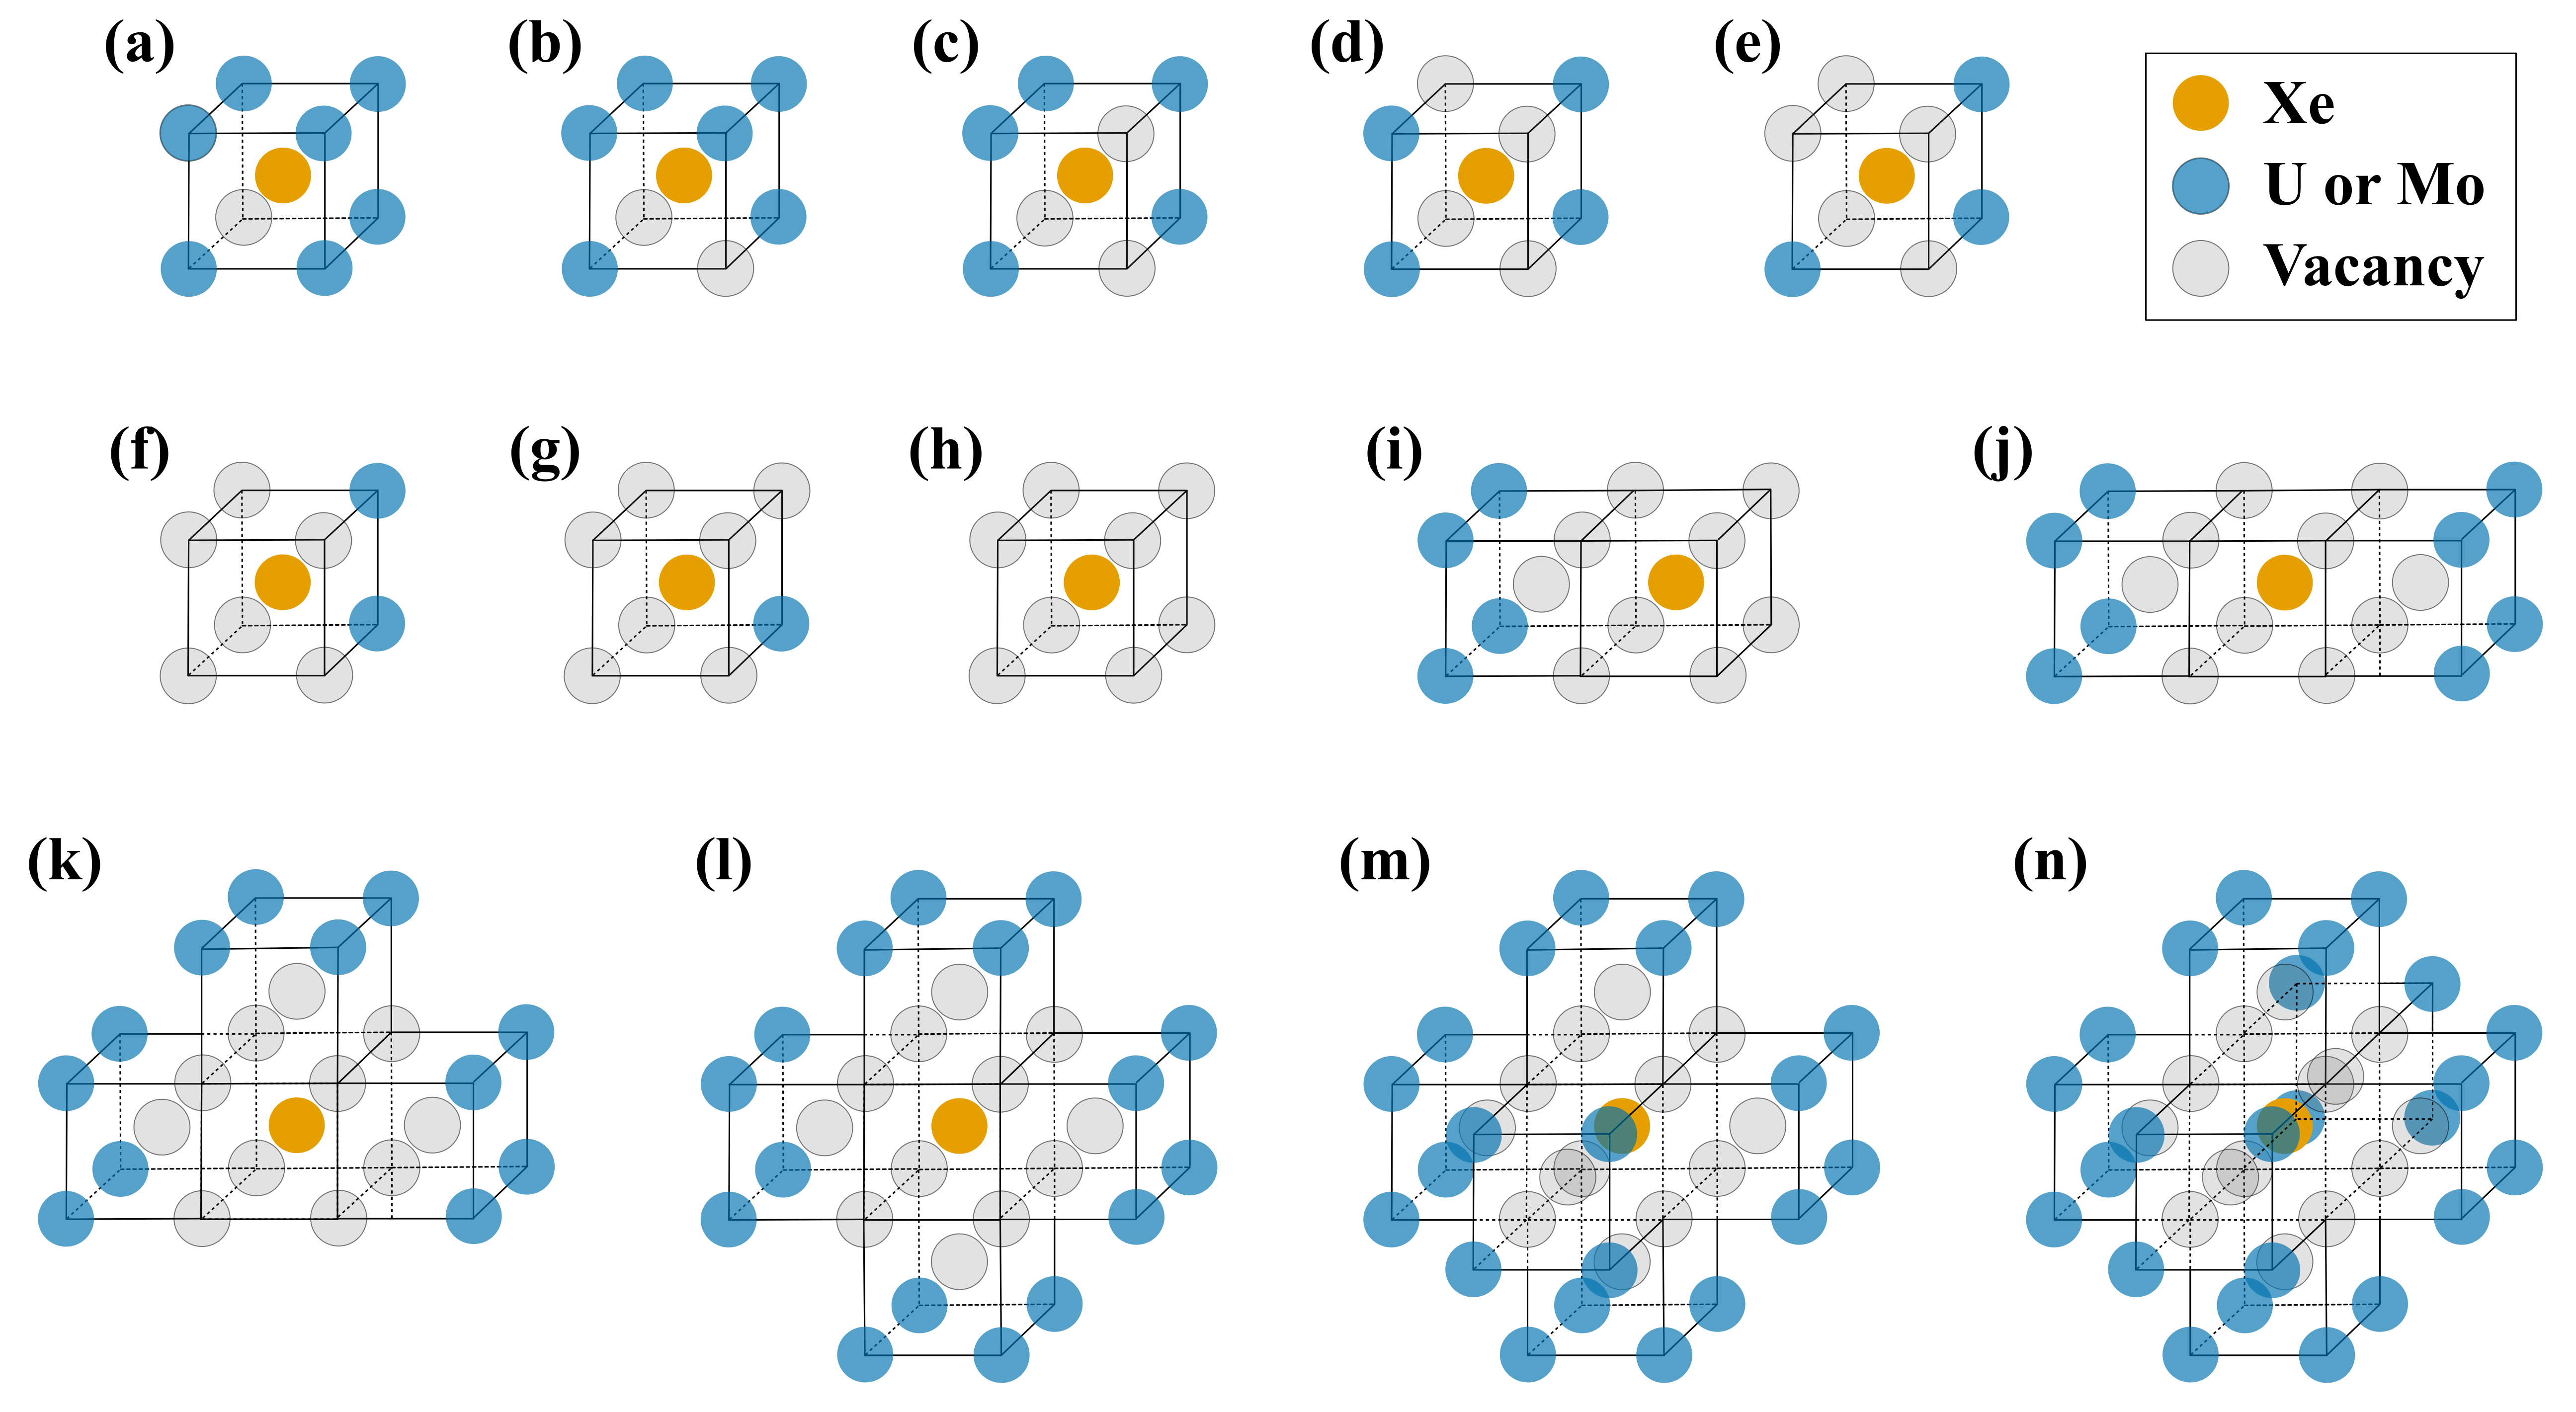
\includegraphics[width=1.0\textwidth]{Fig1.png}
\caption{Schematics of the Xe-vacancy clusters in $\gamma$U-10Mo considered in the present work: (a) Xe-monovacancy ($\it{n}$=1), (b) Xe-divacancy ($\it{n}$=2), (c) Xe-trivacancy ($\it{n}$=3), (d) Xe-quadvacancy ($\it{n}$=4), (e) Xe-pentavacancy ($\it{n}$=5), (f) Xe-hexavacancy ($\it{n}$=6), (g) Xe-heptavacancy ($\it{n}$=7), (h) Xe-octavacancy ($\it{n}$=8), (i) Xe-nonavacancy ($\it{n}$=9), (j) Xe-decavacancy ($\it{n}$=10), (k) Xe-undecavacancy ($\it{n}$=11), (l) Xe-dodecavacancy ($\it{n}$=12), (m) Xe-tridecavacancy ($\it{n}$=13), and (n) Xe-tetradecavacancy ($\it{n}$=14), where $\it{n}$ is the number of vacancies in a Xe cluster. Blue spheres represent the matrix U-Mo, yellow spheres represent Xe, and grey spheres represent vacant sites. }
\label{fig:xeclusters}
\end{figure}

\subsection{Steady-State Defect Concentration under Irradiation}
The steady-state concentration of vacancies and interstitials under irradiation conditions can be obtained by solving the coupled differential equations as follows:

\begin{align} 
\label{eqn:UMoratetheory1}
\frac{dC_{v}}{dt}={}&\epsilon\dot{F}- K_{iv}C_{i}C_{v} - k_{vs}^{2}D_{v}C_{v}, \\
\notag\\
\label{eqn:UMoratetheory2}
\frac{dC_{i}}{dt}={}&\epsilon\dot{F} - K_{iv}C_{i}C_{v} - k_{is}^{2}D_{i}C_{i}, 
\end{align}

\noindent where $C_{v}$ is the concentration of vacancies, $C_{i}$ is the concentration of interstitials, $\epsilon$ is the defect production rate per fission event, $K_{iv}$ is the recombination rate constant between vacancies and interstitials, $k_{vs}^{2}$ is the sink strength of grain boundaries for vacancies, $k_{is}^{2}$ is the sink strength of grain boundaries for interstitial atoms, $D_{v}$ is the vacancy diffusion coefficient, and $D_{i}$ is the interstitial diffusion coefficient. Sinks were restricted to grain boundaries in this work (e.g., dislocation sinks were neglected). The coupled differential equations were solved using the Rosenbrock solver (Rodas-4) with Julia \cite{wanner1996solving, bezanson2017julia}.\\ 
\indent The defect production rate ($\epsilon$) was calculated from the athermal recombination corrected dpa (arc-dpa) model \cite{nordlund2018improving}, which is a modification of the NRT dpa model \cite{norgett1975proposed} which calculates the number of atomic displacements. The arc-dpa model takes into account thermally activated recombination, resulting in a decrease in the number of defects existing under irradiation as compared to the NRT dpa model \cite{nordlund2018improving}. The number of defects generated ($N_{d}$) is described by the arc-dpa model as:\\

\begin{equation}
N_{d} = \frac{0.8T_{d}}{2E_{d}}\xi,
\end{equation}
\\
\noindent where $T_{d}$ is the damage energy, $E_{d}$ is the threshold displacement energy, and $\xi$ is the arc-dpa efficiency function \cite{nordlund2018improving}. The damage energy is taken as the kinetic energy of the fission fragments produced from a fission reaction (approximately 170 MeV), and reduced to account for electronic energy losses. It is assumed that only ballistic effects generate Frenkel pairs. The electronic energy losses have been previously calculated to be 95$\%$, thus the damage energy used is 8.5 MeV \cite{beeler2021radiation}. The magnitude of the threshold displacement energy for $\gamma$U-10Mo is not well known, but can potentially be determined from MD simulations or from experiments. Given that such studies are beyond the scope of this work, reasonable approximations are made for the threshold displacement energy (60 eV) based upon MD simulations in $\gamma$U \cite{beeler2018calculation}, and for the arc-dpa efficiency (0.25), which is approximately the same as bcc Fe \cite{nordlund2018improving}. This yields approximately 14,000 point defects per fission event in $\gamma$U-10Mo. The defect production rate was obtained by dividing the number of generated defects per fission event by the atomic number density of $\gamma$U-10Mo. Any bias towards interstitial atoms or vacancies in the defect production process is neglected, assuming that an equal number of both types of defects are generated. The number of point defects generated in a fission event for this work utilized calculations from Beeler et al. \cite{beeler2021radiation}, which generally agreed with the estimates from Kolotova et al. \cite{kolotova2019atomistic}. \\
\indent In order to determine the recombination rate constant ($K_{iv}$), separate MD simulations were conducted. A supercell of 40 x 40 x 40 unit cells (128,000 atoms) of $\gamma$U was generated with an atomic composition of 10 wt.$\%$ of Mo with periodic boundary conditions. Fifty Frenkel pairs were created, ensuring that the distance between individual defects is at least 4a$_{0}$, where $a_{0}$ is the lattice constant. The system was equilibrated for 20,000 timesteps with a variable timestep such that a maximum distance for an atom to move in one timestep is 5 fm, in order to perform a constrained relaxation of the defects. Subsequently, the system was evolved for 10 ns with a timestep of 1 fs, tracking the number of Frenkel pairs as a function of time via the Voronoi occupation methodology within the LAMMPS. This computational setup is in line with previous efforts to determine recombination rate constants utilizing MD \cite{zhang2012atomistic}. This defect evolution simulation was performed from 600 K to 1200 K in increments of 100 K. For a given temperature, the number of defects ($C_{0}$) as a function of time can be fit to C = $C_{0}/(C_{0}K_{iv}t +1)$, where $C_{0}$ is the initial concentration of Frenkel pairs. In classical rate theory, the grain boundaries are constant sinks and their strength, $k^{2}$, is estimated as 15/$L^{2}$ (L is the grain size, in units of nm) for grain boundaries with a regular pattern, and is identical for both interstitials and vacancies. This assumption is utilized here as a first approximation, and along with a grain size estimate of \SI{10}{\micro\metre}, completes the parameterization of the rate theory equations. The grain size is defined as the average diameter of the grains. It should be noted that the steady-state concentration of defects increased with increasing grain size, and saturated when the grain size was greater than \SI{1}{\micro\metre}. \\

\subsection{Xe-Vacancy Cluster Concentration under Irradiation}

\indent A separate rate-theory formulation was constructed with the assumption that Xe, the most common fission product \cite{kleykamp1985chemical}, was continuously produced in the system, and thus Xe-vacancy clusters with various sizes were also present. Xe-vacancy clusters containing up to fourteen vacancies were taken into account, as mentioned previously. For instance, the first and second nearest neighbor shells are completely composed of vacancies near a Xe atom within a bcc lattice in a Xe-tetravacancy cluster ($\it{n}$=14). The rate of change in defect concentrations including Xe and Xe-vacancy clusters with time can be mathematically described as follows:

\begin{align} 
\label{eqn:Xe_rate1}
\frac{dC_{v}}{dt}={}&\epsilon\dot{F}- K_{iv}C_{i}C_{v} - k_{vs}^{2}D_{v}C_{v} \\
&+\sum_{n=1}^{14} \alpha_{n+1}C_{Xe-nv} -\sum_{n=1}^{13} \beta_{n}C_{v}C_{Xe-(n-1)v} + \sum_{n=1}^{13} nRC_{Xe-nv},\notag\\
\
\label{eqn:Xe_rate2}
\frac{dC_{i}}{dt}={}&\epsilon\dot{F} - K_{iv}C_{i}C_{v} - k_{is}^{2}D_{i}C_{i}, 
\\
\label{eqn:Xe_rate3}
\frac{dC_{Xe}}{dt}={}&\tau\dot{F} - \beta_{1}C_{v}C_{Xe} + \alpha_{2}C_{Xe-1v} + \sum_{n=1}^{14} RC_{Xe-nv},\\
\label{eqn:Xe_rate4}
\frac{dC_{Xe-1v}}{dt}={}&\beta_{1}C_{v}C_{Xe} - \beta_{2}C_{v}C_{Xe-1v} - \alpha_{2}C_{Xe-1v} + \alpha_{3}C_{Xe-2v} - RC_{Xe-1v},
\\
\label{eqn:Xe_rate5}
\frac{dC_{Xe-2v}}{dt}={}& \beta_{2}C_{v}C_{Xe-1v} - \beta_{3}C_{v}C_{Xe-2v} - \alpha_{3}C_{Xe-2v} + \alpha_{4}C_{Xe-3v} - RC_{Xe-2v}, 
\\
\label{eqn:Xe_rate6}
\frac{dC_{Xe-3v}}{dt}={}& \beta_{3}C_{v}C_{Xe-2v} - \beta_{4}C_{v}C_{Xe-3v} - \alpha_{4}C_{Xe-3v} + \alpha_{5}C_{Xe-4v} - RC_{Xe-3v},
\\
&\vdotswithin{=} \notag \\
\label{eqn:Xe_rate7}
\frac{dC_{Xe-14v}}{dt}={}& \beta_{14}C_{v}C_{Xe-13v} - \alpha_{15}C_{Xe-14v} - RC_{Xe-14v},
\end{align}

\noindent where $C_{Xe}$ is the Xe concentration, $C_{Xe-nv}$ is the concentration of a Xe cluster containing $\it{n}$ vacancies, $\tau$ is the yield of Xe from fission reactions where $\tau$ = 0.13 \cite{nichols2008handbook}, $\beta_{n}$ is the absorption coefficient, $\alpha_{n}$ is the emission coefficient, and $\it{R}$ is the re-solution rate of a Xe-vacancy cluster where $\it{R}$ = 2.0 $\times$ 10$^{-24}$ $\times$ $\dot{F}$ (s$^{-1}$) \cite{beeler2021microstructural}. The absorption and emission coefficients were calculated by Eqns. \ref{eq:beta} and \ref{eq:alpha} \cite{bai2017modeling}:\\

\begin{equation}
\label{eq:beta}
\beta_{n} = \frac{4\pi(r_{0}+r_{n})D_{v}}{V_{at}},
\end{equation}

\begin{equation}
\label{eq:alpha}
\alpha_{n+1} = \beta_{n}\textrm{exp}(\frac{-E_{n+1}^{b}}{kT}),
\end{equation}
\\
\noindent where $r_{0}$ is the radius of a single vacancy, $r_{n}$ is the radius of a Xe-vacancy cluster containing $\it{n}$ vacancies, and $E_{n}^{b}$ is the binding energy of the $\it{n}^{th}$ vacancy in a Xe cluster containing $\it{n}$ vacancies. Assuming all clusters are spherical, $r_{n}$ = $(\frac{3nV_{at}}{4\pi})^{1/3}$, where $V_{at}$ is the volume per atom for the bcc crystal structure, given by $V_{at}$ = $\frac{a_{0}^3}{2}$. The binding energy of the $\it{n}^{th}$ vacancy in a Xe cluster containing $\it{n}$ vacancies ($E^{b}_{n}$) was calculated as in Eqn. \ref{eq:be}:\\

\begin{equation}
\label{eq:be}
E^{b}_{n} = E^{f}_{Xe-(n+1)vac} - E^{f}_{Xe-nvac} - E^{f}_{v},
\end{equation}
\\
\noindent where $E^{f}_{Xe-nvac}$ is the formation energy of a Xe cluster containing $\it{n}$ vacancies, $E^{f}_{Xe-(n+1)vac}$ is the formation energy of a Xe cluster containing $\it{n}$+1 vacancies, and $E^{f}_{v}$ is the vacancy formation energy. The vacancy formation energy in $\gamma$U-10Mo was assumed to be 1.6 eV \cite{beeler2020improved}.\\ 
\indent Separate MD simulations were also performed to calculate the formation energies of a Xe-vacancy cluster in $\gamma$U-10Mo. A supercell of 10 x 10 x 10 unit cells of $\gamma$U was created with periodic boundary conditions. Twenty-three percent of the U atoms in the system were substituted by Mo atoms to produce $\gamma$U-10Mo. The system was equilibrated for 200 ps at the evaluated temperatures (from 400 K to 1400 K in increments of 200 K) in an NPT ensemble with a Langevin thermostat in the Gronbech-Jenson-Farago formalism \cite{gronbech2013simple, gronbech2014application} with a timestep of 0.002 ps. Subsequently, various sizes of the Xe-vacancy clusters were created in the system separately (Fig. \ref{fig:xeclusters}), and the system was equilibrated for another 200 ps. The formation energies of a Xe cluster containing $\it{n}$ and $\it{n}$+1 vacancies ($E_{Xe-nvac}^{f}$ and $E_{Xe-(n+1)vac}^{f}$) were calculated as in Eqns. \ref{eq:eform1} and \ref{eq:eform2}:\\

\begin{equation}
\label{eq:eform1}
E_{Xe-nvac}^{f} = E_{Xe-nvac} - \frac{\{N-(n+1)\}}{N}E_{ideal}, 
\end{equation}

\begin{equation}
\label{eq:eform2}
E_{Xe-(n+1)vac}^{f} = E_{Xe-(n+1)vac} - \frac{\{N-(n+2)\}}{N}E_{ideal}, 
\end{equation}
\\
\noindent where $\it{E}_{ideal}$ is the potential energy of the system containing no defects, $\it{E}_{Xe-nvac}$ is the potential energy of the system containing a Xe cluster with $\it{n}$ vacancies, $\it{E}_{Xe-(n+1)vac}$ is the potential energy of the system containing a Xe cluster with $\it{n}$+1 vacancies, and $\it{N}$ is the number of atoms in the system. Numerous simulations were conducted until the cumulative moving average of the potential energy of each system converged to consider different configurational environments (U and Mo) in the alloy \cite{park2021atomistic}. Thus, two hundred simulations were performed, and the potential energies were averaged at each temperature.
\\

\subsection{Radiation-enhanced Diffusion of U, Mo, and Xe in $\gamma$U-10Mo}
Given a steady-state concentration of vacancies and interstitials under irradiation and the diffusion coefficients of vacancies and interstitials, the radiation-enhanced diffusion coefficient $(D_{RED})$ of U and Mo can be expressed as follows \cite{was2016fundamentals}:

\begin{equation}
D_{RED}^{U}= D_{v}^{U}C_{v}^{irr} + D_{i}^{U}C_{i}^{irr},
\end{equation}

\begin{equation}
D_{RED}^{Mo}= D_{v}^{Mo}C_{v}^{irr} + D_{i}^{Mo}C_{i}^{irr},
\end{equation}
\\
\noindent where $D^{U}_{v}$ is the vacancy diffusion coefficient of U, $D^{Mo}_{v}$ is the vacancy diffusion coefficient of Mo, $D^{U}_{i}$ is the interstitial diffusion coefficient of U, $D^{Mo}_{i}$ is the interstitial diffusion coefficient of Mo, $C^{irr}_{v}$ is the steady-state concentration of vacancies under irradiation, and $C^{irr}_{i}$ is the steady-state concentration of interstitials under irradiation. Unlike U and Mo, it is assumed that the diffusion of Xe occurs through vacancy clustering, and thus the radiation-enhanced diffusion coefficient of Xe can be described as follows \cite{was2016fundamentals}:\\
\begin{equation}
D^{Xe}_{RED} = \sum_{n=1}^{k-1} D_{nvac}^{Xe}C_{Xe-nvac}^{irr},
\end{equation}
\\
\noindent where and $C_{Xe-nvac}^{irr}$ is the concentration of a Xe cluster containing $\it{n}$ vacancies under irradiation. It was assumed that Xe-vacancy clusters do not interact with each other. As will be discussed, in order to approximate losses to large bubbles, the largest Xe-vacancy clusters are considered immobile.

\subsection{Intrinsic Thermal Diffusion of Xe in $\gamma$U-10Mo}
The intrinsic thermal diffusion coefficient of Xe in $\gamma$U-10Mo was also calculated since both experimental and computational data do not exist. In addition, the previously utilized value of the intrinsic thermal diffusion coefficient of Xe is based on the hypothesis that the intrinsic thermal diffusion of Xe is slower than that of U by four orders of magnitude \cite{hu2016formation}. 
With the assumption that diffusion of Xe is mediated by a vacancy \cite{perriot2019atomistic, andersson2019density, andersson2011u, thompson2013pathway, bes2015experimental}, the intrinsic thermal diffusion of Xe ($D^{Xe^{2}}_{INT}$) can be calculated under the same computational parameters described in Section \ref{sec:DC_UMoXe} as follows:
\\
\begin{equation}
D^{Xe^{2}}_{INT} = c_{v}D_{1vac}^{Xe},
\end{equation}
\\
where $c_{v}$ is the vacancy concentration at equilibrium and $D_{1vac}^{Xe}$ is the diffusion coefficient of Xe in a mono-vacancy cluster. The concentration of vacancies at equilibrium was calculated using the equation as follows:

\begin{equation}
\label{eq:surface}
c_{v}=exp\left({\frac{\Delta S_{v}^{f}}{k_{B}}}\right) exp\left({\frac{-E_{v}^{f}}{k_{B}T}}\right),
\end{equation}

\noindent where $\Delta S^{f}_{v}$ is the change in entropy introduced from creating a vacancy. The equilibrium vacancy concentration is not affected by the entropy term, as has been previously assumed in diffusional studies in $\gamma$U-Mo \cite{park2021atomistic, smirnova2015investigation}.

\section{Results}
\subsection{Recombination Rate Constant}\label{sec:recomb}
The number of defects was determined as a function of time in the temperature range between 600 K and 1200 K in increments of 100 K. Fig. \ref{fig:recomb}(a) represents the defect concentration with respect to time in $\gamma$U-10Mo at 1000 K, as an example. Temperatures below 600 K were not explored, as intrinsic diffusion on MD timescales is very limited below 600 K in $\gamma$U-10Mo.  It can be observed that the number of defects decays as a function of time in a near-exponential fashion, with the rate of annihilation slowing as a function of time due to the decreased number of defects present. The fit to the data is also shown in Fig. \ref{fig:recomb}(a), which provides a value of the recombination rate constant ($K_{iv}$) at 1000 K. For each individual temperature analyzed, the recombination rate constant is calculated from the defect concentration as a function of time. Fig. \ref{fig:recomb}(b) represents the recombination rate constant from 600 K to 1200 K along with the power function fit.\\
\indent According to kinetic theory \cite{was2016fundamentals}, the recombination rate constant can be estimated as $K_{iv}$ =4$\pi$($D_{v}$+$D_{i}$)$r_{iv}$/$V_{at}$, where $r_{iv}$ is the interstitial-vacancy recombination radius. Typical values of the recombination radius are on the order of 2-3 times the equilibrium lattice constant ($a_{0}$) \cite{yu2012radiation, nakashima2015recombination}. By utilizing the fit values of the recombination rate constant and the known diffusion coefficients and equilibrium volume, the recombination radius can be determined. It is found that the recombination radius is significantly larger than what is typically observed. For example, at 1000 K, the recombination radius is approximately 8$a_{0}$. As the temperature decreases, the recombination radius increases farther, such that the distance of the recombination radius at 600 K is 24$a_{0}$. Considerably larger recombination radii (3.5–15$a_{0}$) were also observed in UO$_{2}$, which is in agreement with the present work \cite{veshchunov2015development}. It is assumed that this is due to the long stress field interactions between interstitials and vacancies, leading to rapid recombination. This perhaps compensates for the low interstitial formation energies in $\gamma$U systems, such that the large number of defects that are created can also rapidly recombine. Such a phenomenon was hinted at in previous studies of displacement energies in $\gamma$U \cite{beeler2018calculation}.

\begin{figure}[hbt!]
\centering
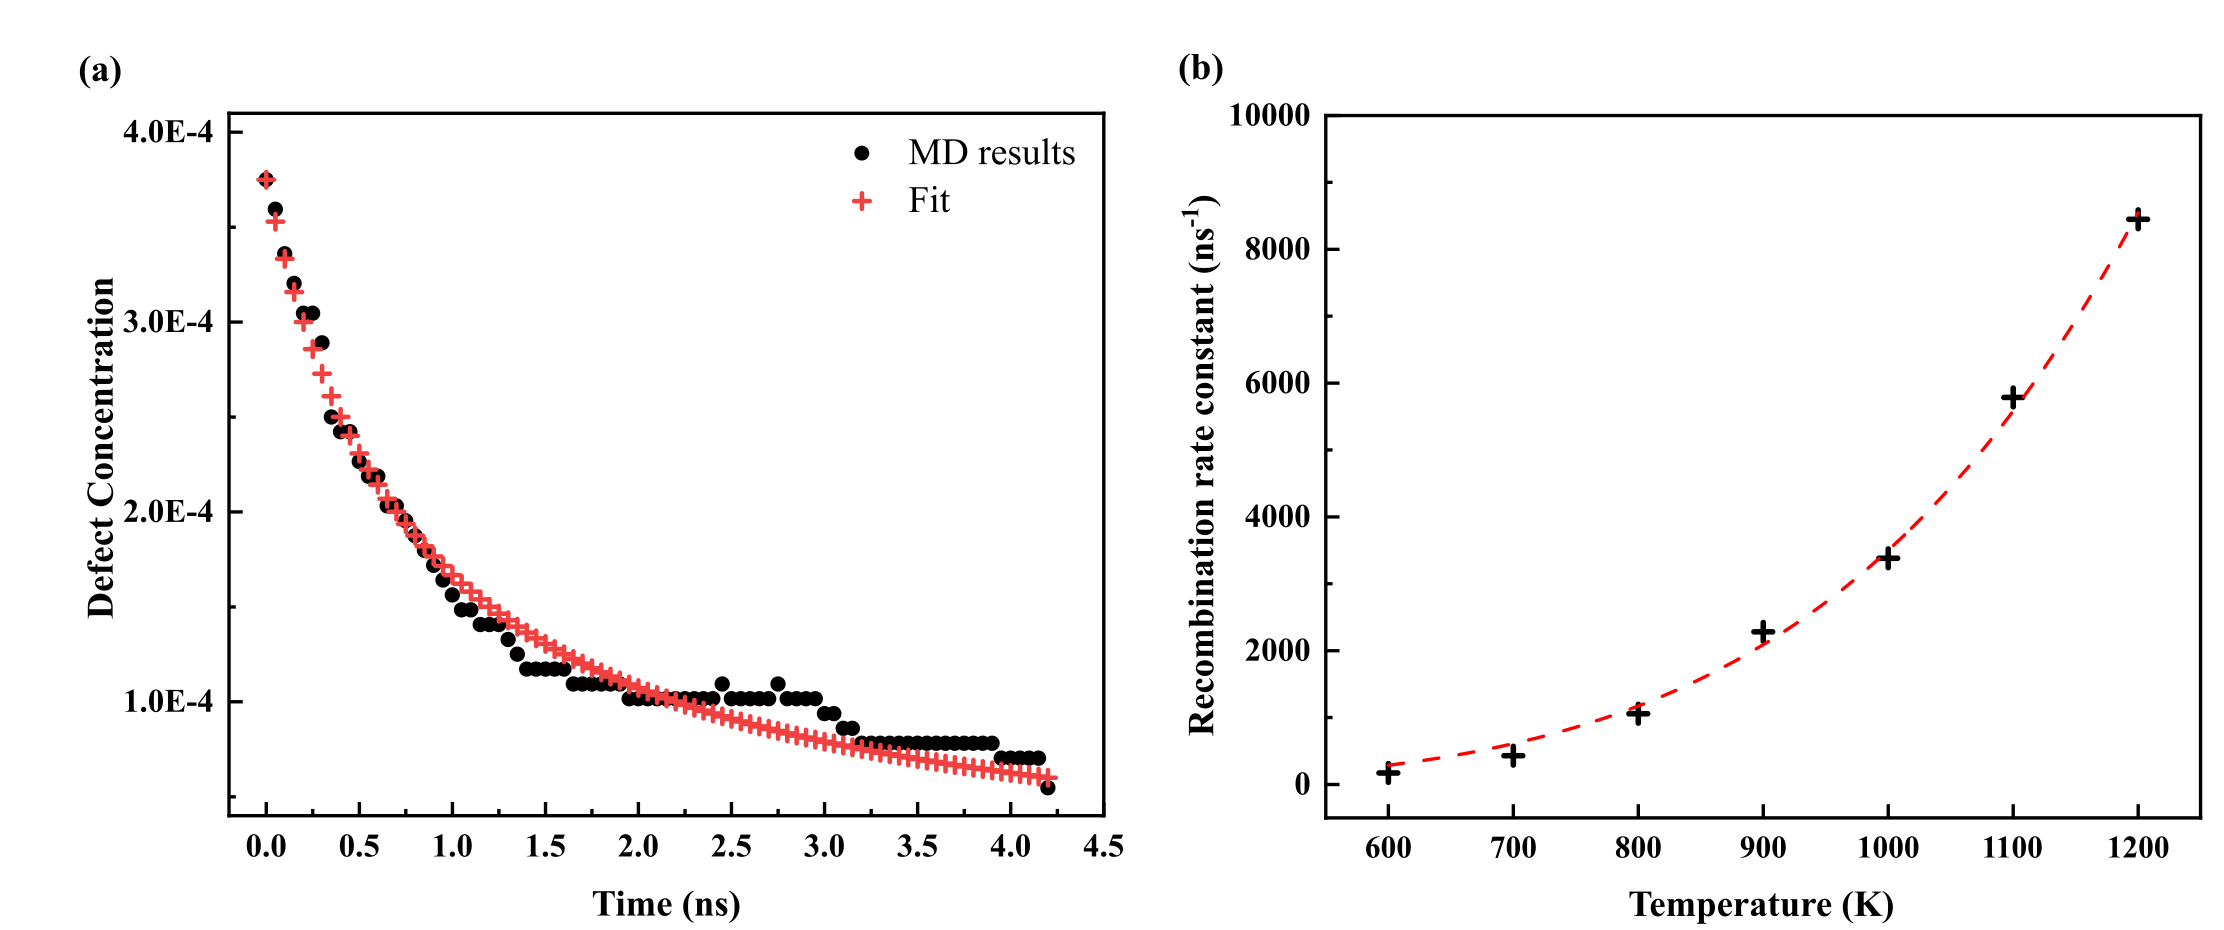
\includegraphics[width=1\textwidth]{Fig2.png}
\caption{(a) The evolution of Frenkel pair concentration as a function of time at 1000 K, accounting for recombination. (b) Recombination rate constants $(\it{K}_{iv})$ as a function of temperature.}
\label{fig:recomb}
\end{figure}

\subsection{Radiation-enhanced Diffusion of U and Mo}\label{sec:RED_UMo}
Implementing the recombination rate constant from Section \ref{sec:recomb}, Eqns. \ref{eqn:UMoratetheory1} and \ref{eqn:UMoratetheory2} are used to determine the steady-state concentration of point defects under irradiation as a function of temperature in $\gamma$U-10Mo at three different fission rate densities. Fig. \ref{fig:def_conc}(a) shows the evolution of the concentration of vacancies and interstitials at the fission rate density of 5$\times$10$^{20}$ fiss/m$^{3}$/s at 1000 K, as an example. It took approximately 0.2 s for the concentration of both vacancies and interstitials to reach steady-state under these conditions. With decreasing temperature, it takes longer for the concentrations of vacancies and interstitials to reach the steady-state, as expected. The steady-state concentrations of vacancies and interstitials as a function of temperature are shown at three different fission rate densities in Fig. \ref{fig:def_conc}(b). As the temperature increases, the number of vacancies and interstitials recombining increases, resulting in a decrease in the steady-state concentration of vacancies and interstitials. The concentration of vacancies was higher than the concentration of interstitials since the interstitials, which diffuse faster than vacancies, diffused into sinks such as grain boundaries \cite{park2021atomistic, smirnova2015atomistic}. The concentration of vacancies decreased more rapidly than the concentration of interstitials with increasing temperature. This implies that the diffusion of vacancies is more sensitive to temperature than the diffusion of interstitials.

\begin{figure}[hbt!]
\centering
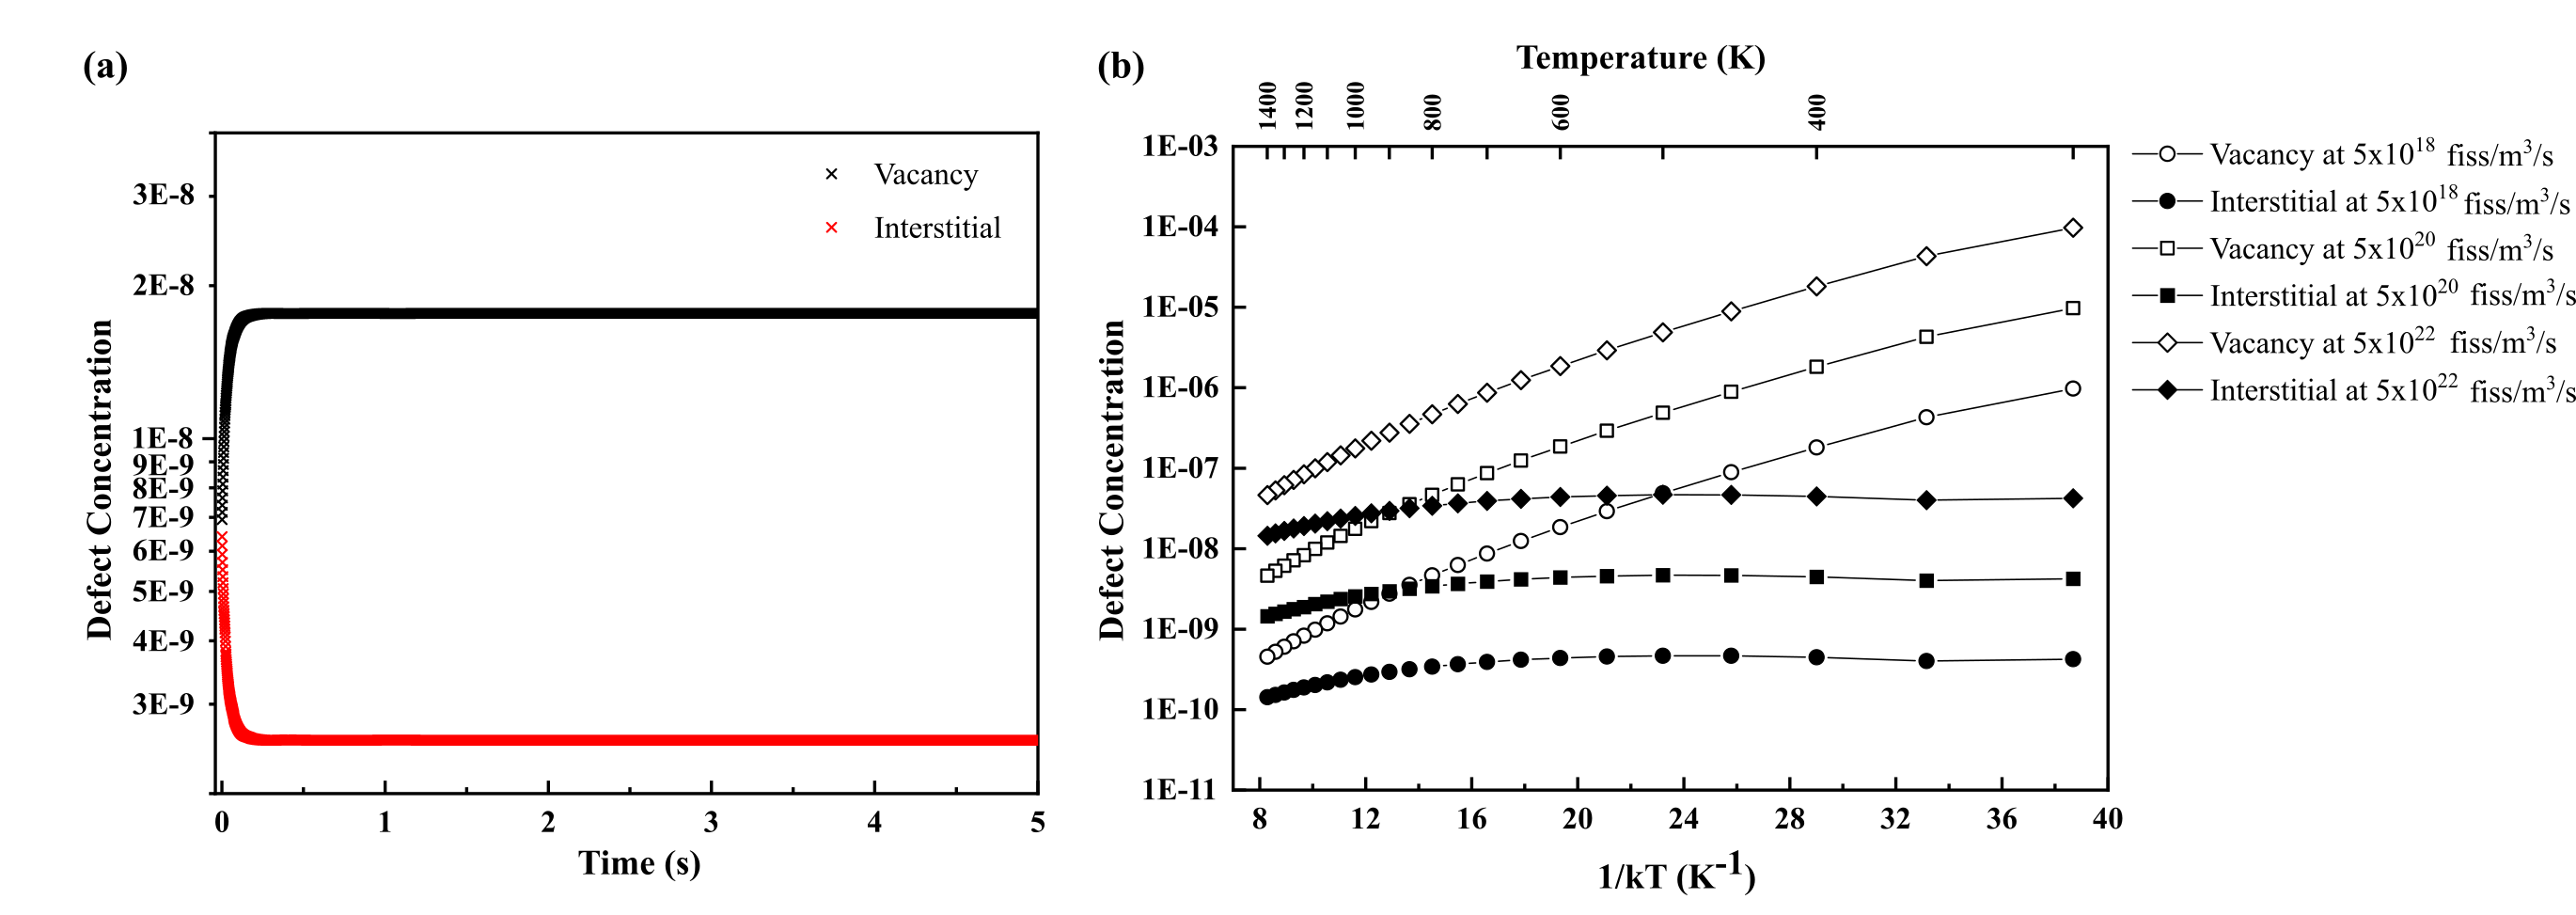
\includegraphics[width=1\textwidth]{Fig3.png}
\caption{(a) Evolution of concentration of vacancies and interstitials as a function of time at the fission rate density of 5$\times$10$^{20}$ fiss/m$^{3}$/s at 1000 K, as an example. (b) Rate theory calculations of the defect concentration evolution as a function of inverse temperature at three fission rate densities (units are fiss/m$^{3}$/s). Note that the y-axis is shown in a log scale.}
\label{fig:def_conc}
\end{figure}

\indent Fig. \ref{fig:diffcoefficient1}(a) shows the vacancy and interstitial diffusion coefficients of U and Mo in $\gamma$U-10Mo as a function of temperature. The calculated diffusion coefficients were extrapolated to lower temperatures by fitting to an Arrhenius equation. The calculation of vacancy and interstitial diffusion of U and Mo ($D^{U}_{v}$, $D^{U}_{i}$, $D^{Mo}_{v}$, and $D^{Mo}_{i}$) in $\gamma$U-10Mo was previously conducted by the authors \cite{park2021atomistic}, and additional MD calculations were conducted at 900 K, 1100 K, 1300 K, and 1400 K to improve statistics within this work. The diffusion via interstitial atoms was faster than diffusion via vacancies in the evaluated temperature range, indicating that the diffusion in $\gamma$U-10Mo takes place primarily via interstitial atoms \cite{park2021atomistic, smirnova2015atomistic}. Vacancy and interstitial diffusion of U and Mo ($D^{U/Mo}_{v}$ and $D^{U/Mo}_{i}$) were insignificant below 900 K and 800 K, respectively, within the MD timescales. The results of the Arrhenius fits for vacancy and interstitial diffusion of U and Mo are given in Table \ref{tab:diff1}.\\
\indent Using the steady-state concentration of vacancies and interstitials, as well as the diffusion coefficients of vacancies and interstitials, the radiation-enhanced diffusion coefficients of U and Mo in $\gamma$U-10Mo were calculated, as shown in Fig. \ref{fig:diffcoefficient1}(b), as a function of temperature at three fission rate densities. The radiation-enhanced diffusion of U was found to be faster than that of Mo, originating from the higher interstitial diffusion coefficient of U. The effect of the fission rate density on radiation-enhanced diffusion of U and Mo was evaluated, and a square root dependence of the radiation-enhanced diffusion coefficient was observed, as expected \cite{cooper2021irradiation, matthews2020cluster}. A coefficient for fission-rate dependence can be obtained by dividing the total radiation-enhanced diffusion by the square root of the fission rate density.Thus, the total diffusion coefficients of U and Mo in $\gamma$U-10Mo, respectively, under irradiation can be obtained by the summation of intrinsic thermal diffusion, radiation-enhanced diffusion, and radiation-driven diffusion as follows:
\\

\begin{align} 
D_{U}={}& 1.28\times10^{-5}\times \mbox{exp}(-\frac{1.76}{kT}) \\ 
&+1.10\times10^{-26}\times \mbox{exp}(-\frac{0.38}{kT})\times \sqrt{\dot{F}} + 1.97\times10^{-41}\times \dot{F}, \notag
\end{align}

\begin{align} 
D_{Mo}={}& 1.62\times10^{-5}\times \mbox{exp}(-\frac{1.97}{kT})\\ 
&+2.10\times10^{-27}\times \mbox{exp}(-\frac{0.39}{kT})\times \sqrt{\dot{F}} + 2.01\times10^{-41}\times \dot{F}. \notag
\end{align}
\\
\begin{figure}[hbt!]
\centering
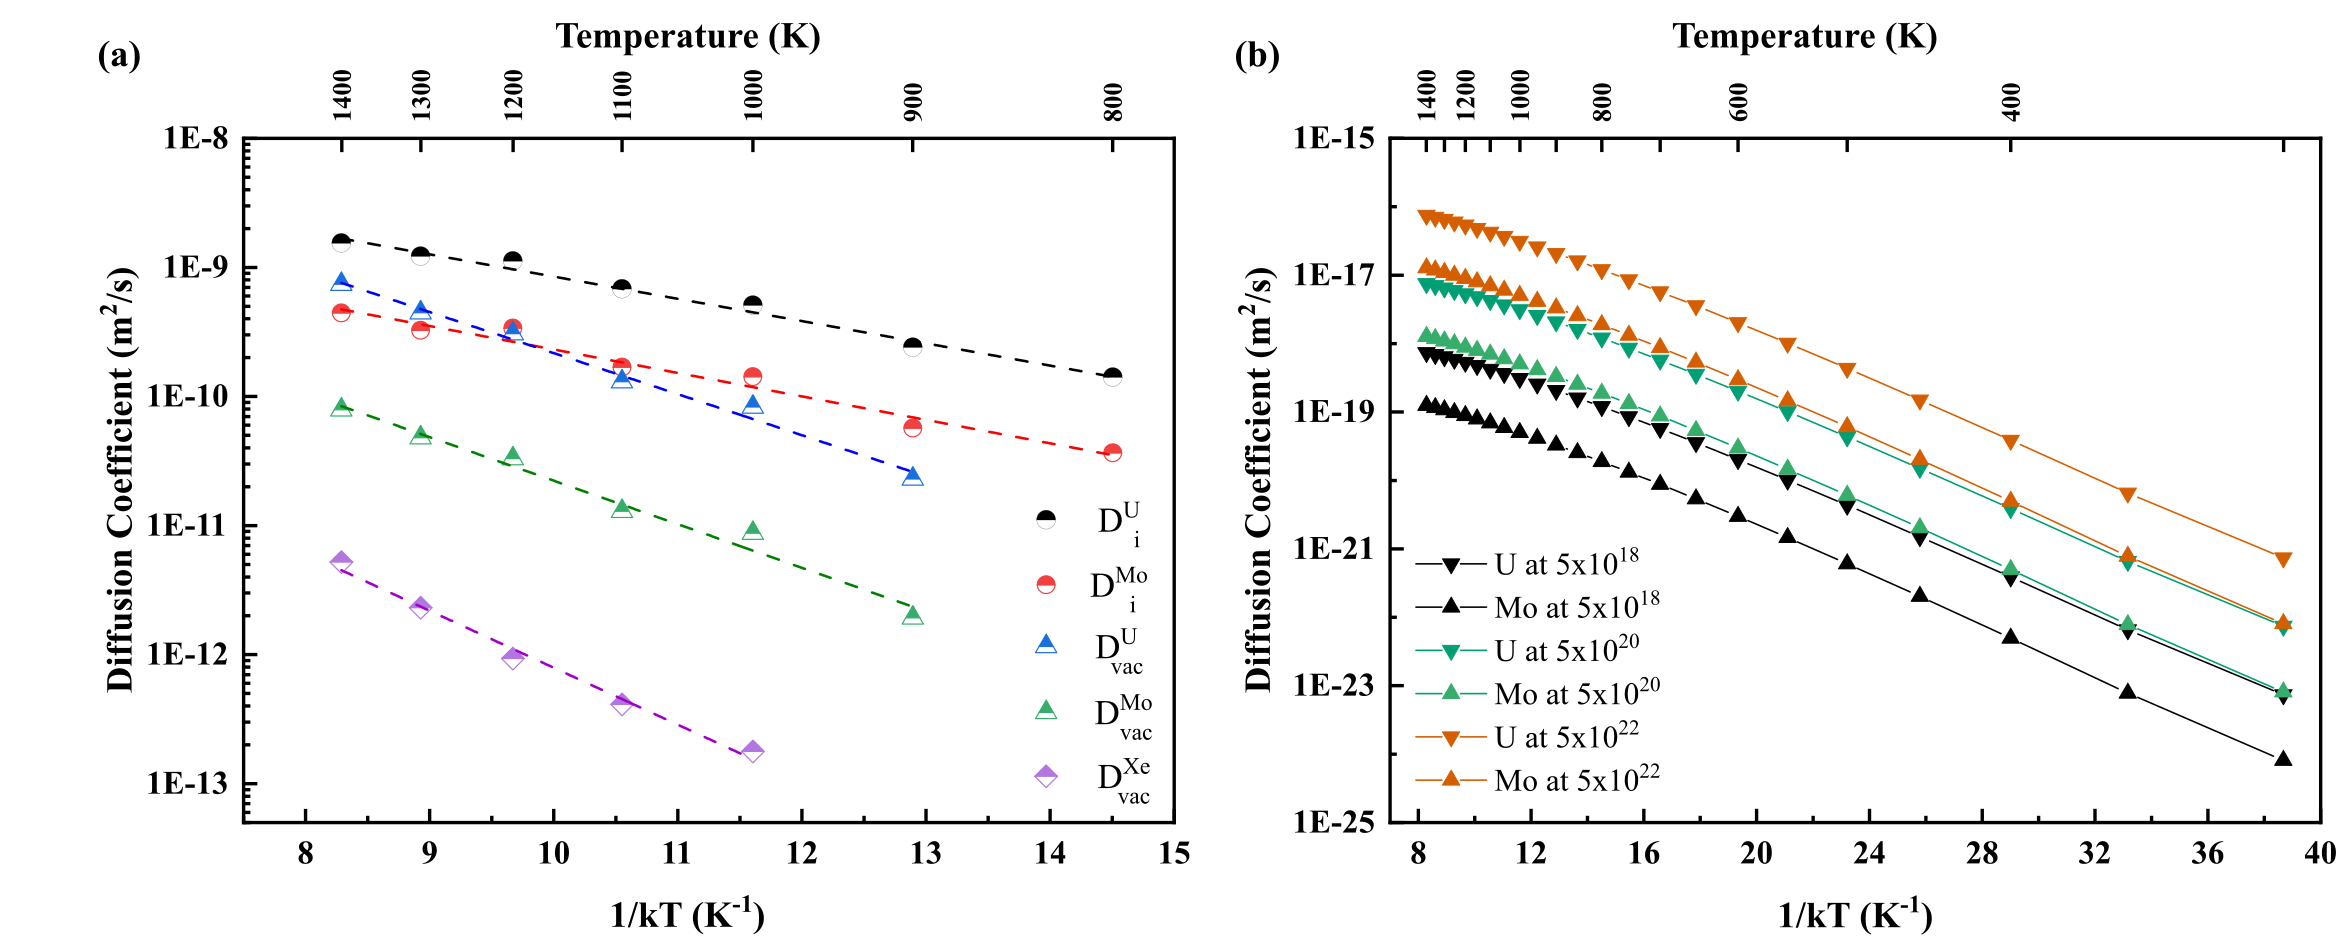
\includegraphics[width=1\textwidth]{Fig4.png}
\caption{(a) Vacancy and interstitial diffusion coefficients of U, Mo, and Xe. (b) Radiation-enhanced diffusion of U and Mo at three fission rate densities (units are fiss/m$^{3}$/s).}
\label{fig:diffcoefficient1}
\end{figure}

\begin{table}[hbt!]
\captionsetup{font=normalsize} 
\caption{Arrhenius fits of vacancy and interstitial diffusion of U, Mo, and Xe in $\gamma$U-10Mo.}
\renewcommand{\arraystretch}{1.2}
\begin{center}
\begin{tabular}{cccc}
\hline
Parameter & Migration energy (eV) & Pre-exponential factor (m$^{2}$/$\mathrm{s}$)  \\ 
\hline
$D^{U}_{i}$ & 0.40 & 4.49$\times$10$^{-8}$ \\  
$D^{Mo}_{i}$& 0.42 & 1.52$\times$10$^{-8}$ \\
$D^{U}_{v}$ & 0.73  & 3.28$\times$10$^{-7}$ \\ 
$D^{Mo}_{v}$& 0.78 & 5.27$\times$10$^{-8}$ \\
$D^{Xe}_{v}$& 1.02 & 2.06$\times$10$^{-8}$ \\
\hline
\end{tabular}
\end{center}
\label{tab:diff1} 
\end{table} 

Radiation-enhanced diffusion of U and Mo in $\gamma$U-10Mo is displayed alongside intrinsic diffusion and radiation-driven diffusion as a function of inverse temperature at three fission rate densities in Fig. \ref{fig:eachU} (a)-(c) and Fig. \ref{fig:eachMo} (a)-(c), respectively. Intrinsic diffusion of U and Mo, calculated via both experiments and MD simulations, are included for comparison purposes \cite{huang2013, park2021atomistic}. The intrinsic diffusion calculated using MD simulations \cite{park2021atomistic}, is significantly higher than the experimental intrinsic diffusion \cite{huang2013}. The disparity in the intrinsic diffusion, determined via experiments \cite{huang2013} and MD simulations \cite{park2021atomistic}, likely originates from the microstructural features. The intrinsic diffusion, calculated via MD simulations, is not affected by the microstructure since the simulations represented an ideal alloy system without defect sinks. Conversely, the experimental results can be influenced by sink features such as dislocations, grain boundaries, and impurities in the alloys, resulting in a decrease in intrinsic diffusion. In addition, in the calculation of intrinsic diffusion using MD simulations \cite{park2021atomistic}, there were only three intrinsic diffusion data points for U and Mo above 800 K since diffusion of U and Mo below 800 K was insignificant within the MD timescale. Thus, the extrapolation using three data points at high temperatures may not be a good assumption for lower temperatures. Therefore, the experimental intrinsic diffusion is utilized for comparison to determine the primary diffusion mechanism during research reactor operating conditions.
\\

When compared to the experimental intrinsic diffusion \cite{huang2013}, the radiation-enhanced diffusion of U and Mo dominated in the intermediate temperature range, depending on the fission rate density. With increasing fission rate densities, the minimum temperature at which radiation-enhanced diffusion dominated increased, and the range of temperatures where radiation-enhanced diffusion is prevalent decreased. Specifically, the radiation-enhanced diffusion of U becomes the primary mode of diffusion between 350 K and 600 K at 5$\times$10$^{18}$ fiss/m$^{3}$/s (Fig. \ref{fig:eachU}(a)), 450 K and 650 K at 5$\times$10$^{20}$ fiss/m$^{3}$/s (Fig. \ref{fig:eachU}(b)), and 550 K and 700 K at 5$\times$10$^{22}$ fiss/m$^{3}$/s (Fig. \ref{fig:eachU}(c)). The radiation-enhanced diffusion of Mo dominated in the temperature ranges between 450 K and 650 K at 5$\times$10$^{18}$ fiss/m$^{3}$/s (Fig. \ref{fig:eachMo}(a)) and 550 K and 700 K at 5$\times$10$^{20}$ fiss/m$^{3}$/s (Fig. \ref{fig:eachMo}(b)). Above the temperature ranges specified, intrinsic thermal diffusion was dominant, while below this temperature range radiation-driven diffusion was dominant. The intrinsic thermal diffusion of Mo became faster than the radiation-enhanced diffusion and the radiation-driven diffusion of Mo above 750 K, and the radiation-driven diffusion of Mo became faster than the intrinsic thermal diffusion and the radiation-enhanced diffusion of Mo below 750 K at 5$\times$10$^{22}$ fiss/m$^{3}$/s (Fig. \ref{fig:eachMo}(c)). This decreasing prevalence of radiation-enhanced diffusion with increasing fission rate density is due to the square-root dependency on the fission rate density, while radiation-driven diffusion exhibits a linear dependency on the fission rate density. Thus, the rate of increase of the radiation-driven diffusion with increasing fission rate density surpasses that of radiation-enhanced diffusion. The total diffusion coefficients of U and Mo (including all three diffusion modes) are represented as a function of inverse temperature at three fission rate densities in Fig. \ref{fig:eachU} (d) and Fig. \ref{fig:eachMo} (d), respectively. 
\\

\begin{figure}[hbt!]
\centering
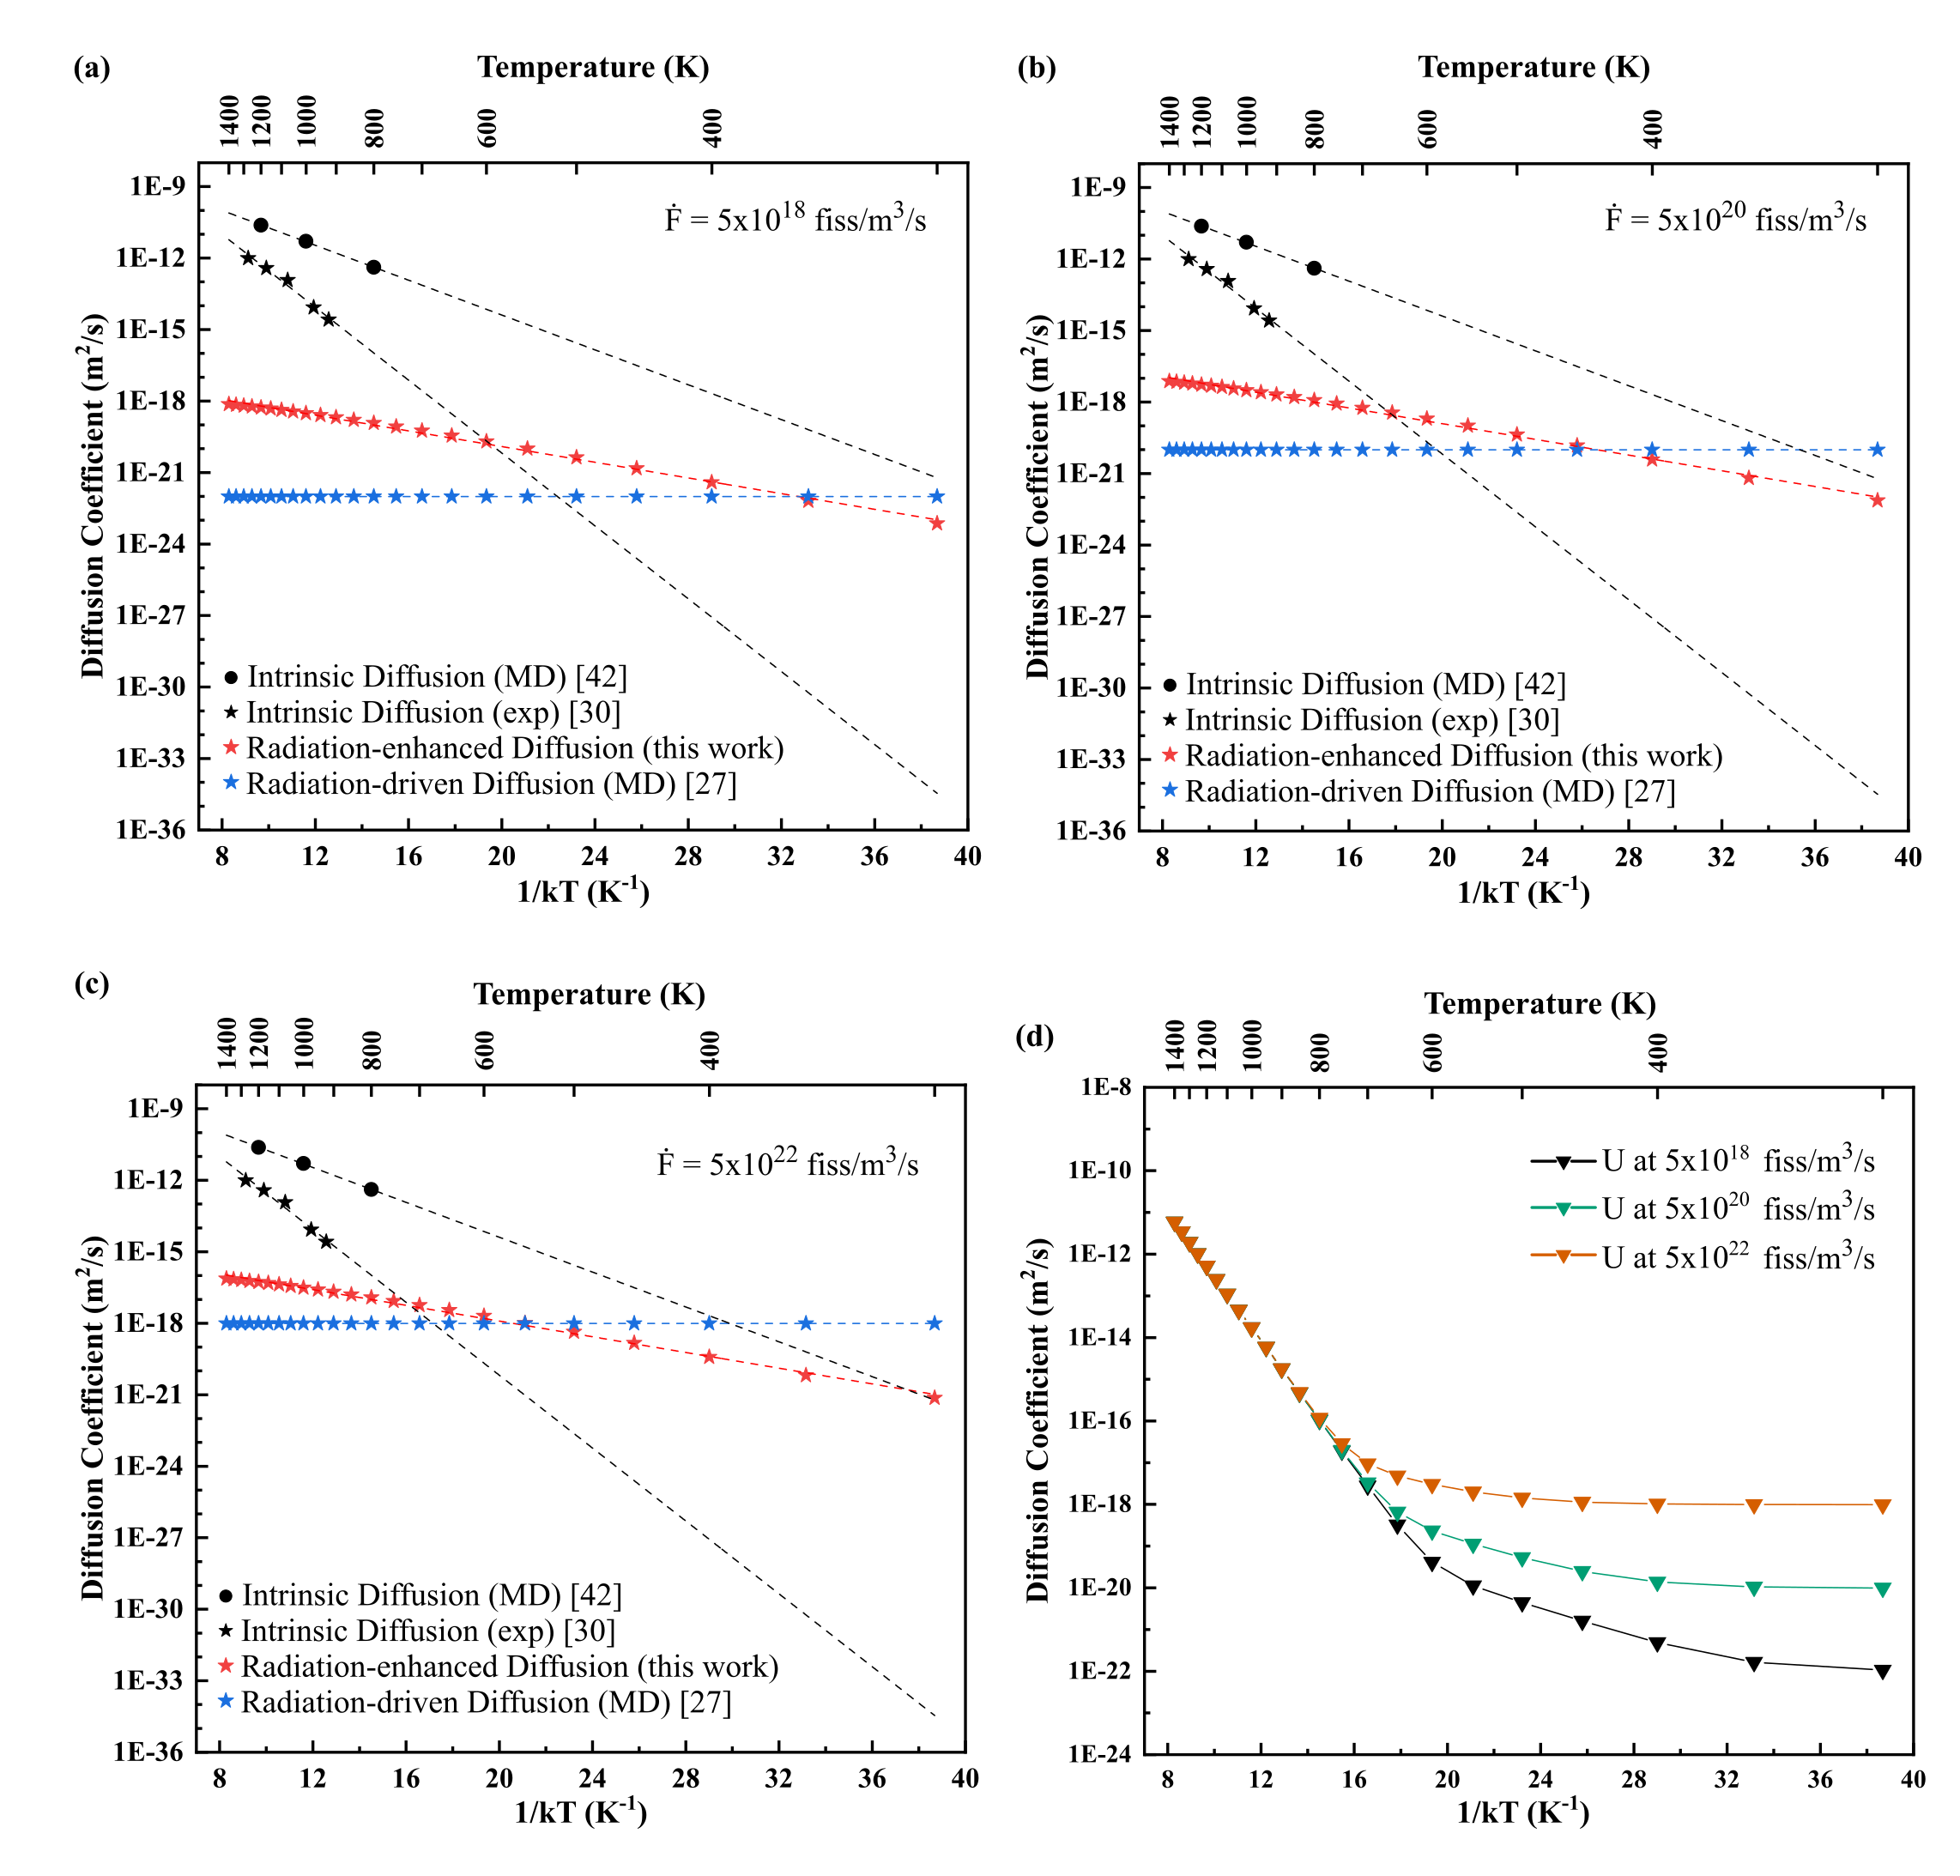
\includegraphics[width=1\textwidth]{Fig5.png}
\caption{Intrinsic diffusion, radiation-enhanced diffusion, and radiation-driven diffusion of U in $\gamma$U-10Mo (a) at 5$\times$10$^{18}$ fiss/m$^{3}$/s, (b) at 5$\times$10$^{20}$ fiss/m$^{3}$/s, and (c) at 5$\times$10$^{22}$ fiss/m$^{3}$/s. (d) Total diffusion of U in $\gamma$U-10Mo at three fission rate densities in fiss/m$^{3}$/s.}
\label{fig:eachU}
\end{figure}

\begin{figure}[hbt!]
\centering
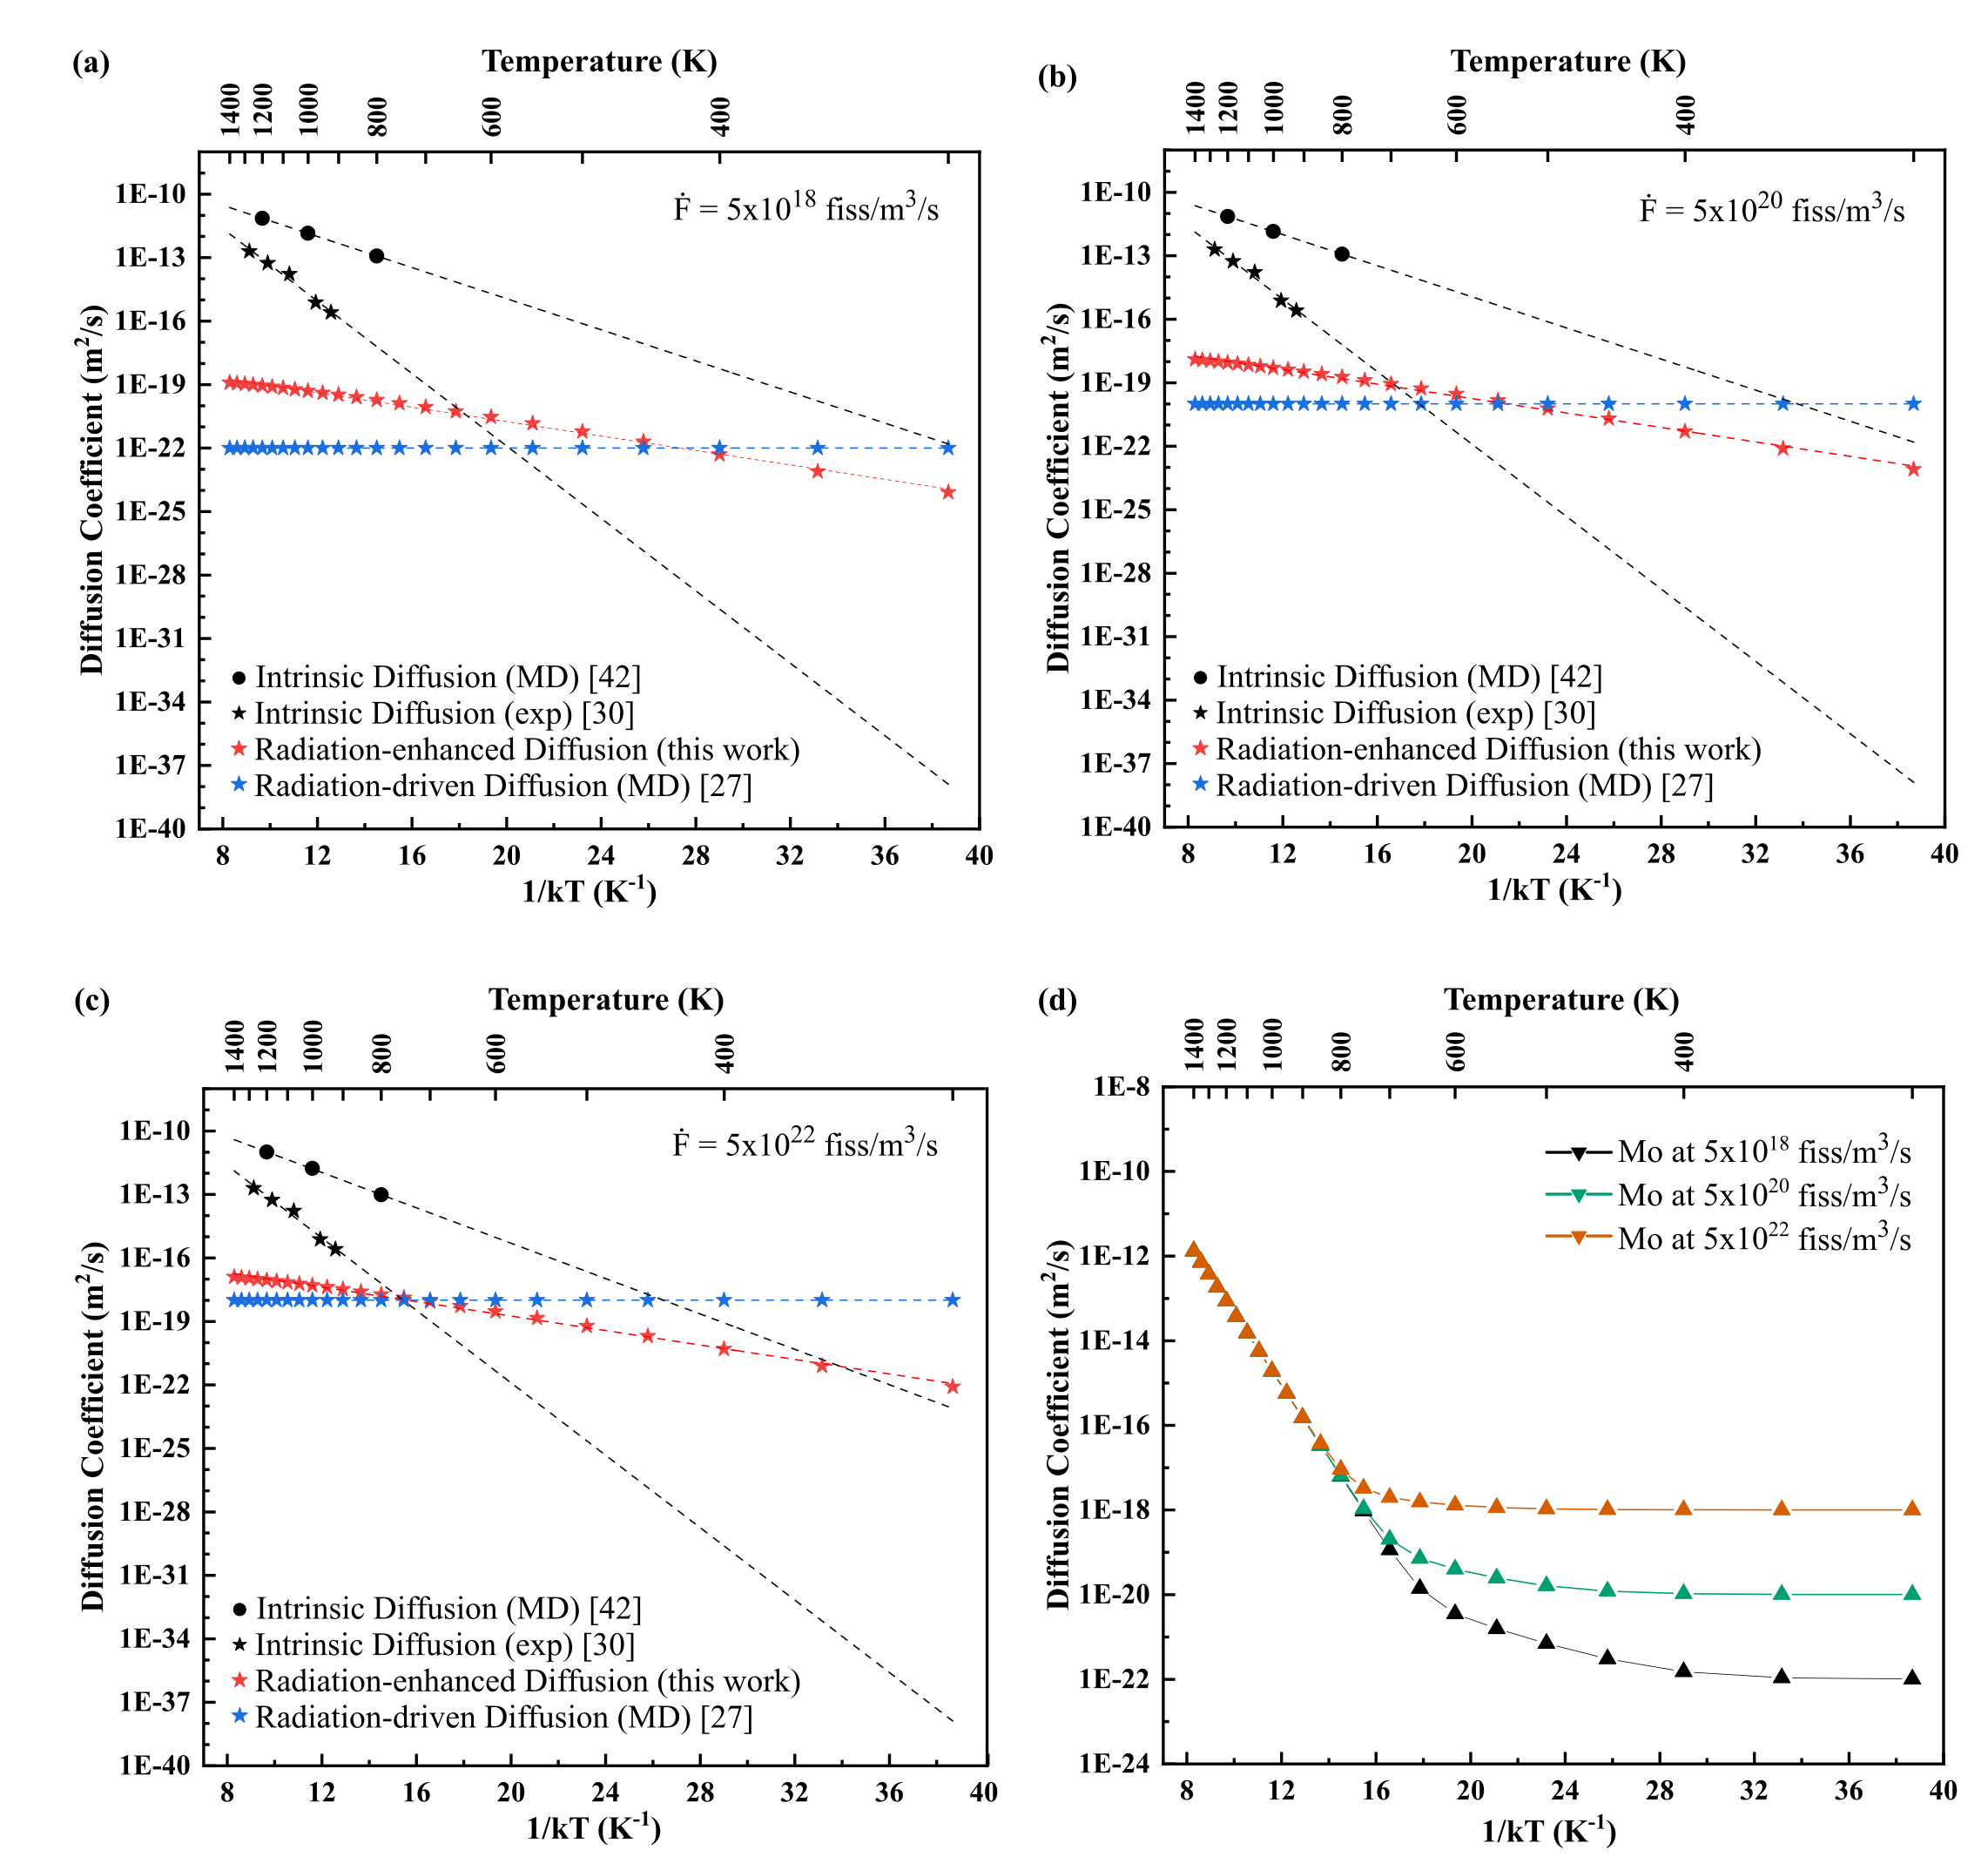
\includegraphics[width=1\textwidth]{Fig6.png}
\caption{Intrinsic diffusion, radiation-enhanced diffusion, and radiation-driven diffusion of Mo in $\gamma$U-10Mo (a) at 5$\times$10$^{18}$ fiss/m$^{3}$/s, (b) at 5$\times$10$^{20}$ fiss/m$^{3}$/s, and (c) at 5$\times$10$^{22}$ fiss/m$^{3}$/s. (d) Total diffusion of Mo in $\gamma$U-10Mo at three fission rate densities in fiss/m$^{3}$/s.}
\label{fig:eachMo}
\end{figure}

\FloatBarrier

\subsection{Radiation-enhanced Diffusion of Xe}
The formation energies of substitutional Xe and Xe-vacancy clusters are calculated as a function of cluster size and temperature as shown in Fig. \ref{fig:FEBE77}(a). The formation energies of the substitutional Xe and the Xe-vacancy clusters increased approximately in a linear fashion with increasing temperature. The formation energy of each Xe-vacancy cluster was fitted linearly, and the binding energies were estimated from the fit value of the formation energies. The estimated binding energy of the $\it{n}^{th}$ vacancy in a Xe cluster with $\it{n}$ vacancies is represented with respect to the Xe cluster size at 1000 K in Fig. \ref{fig:FEBE77}(b), where n = 1, 2, 3, and 4, as an example. The binding energies of the $\it{n}^{th}$ vacancy in a Xe cluster with $\it{n}$ vacancies became higher (more negative) with increasing Xe-vacancy cluster sizes. The binding energy of a Xe cluster containing more than four vacancies was estimated using a linear fit at each temperature from 300 K to 1400 K in increments of 50 K. 

\begin{figure}[hbt!]
\centering
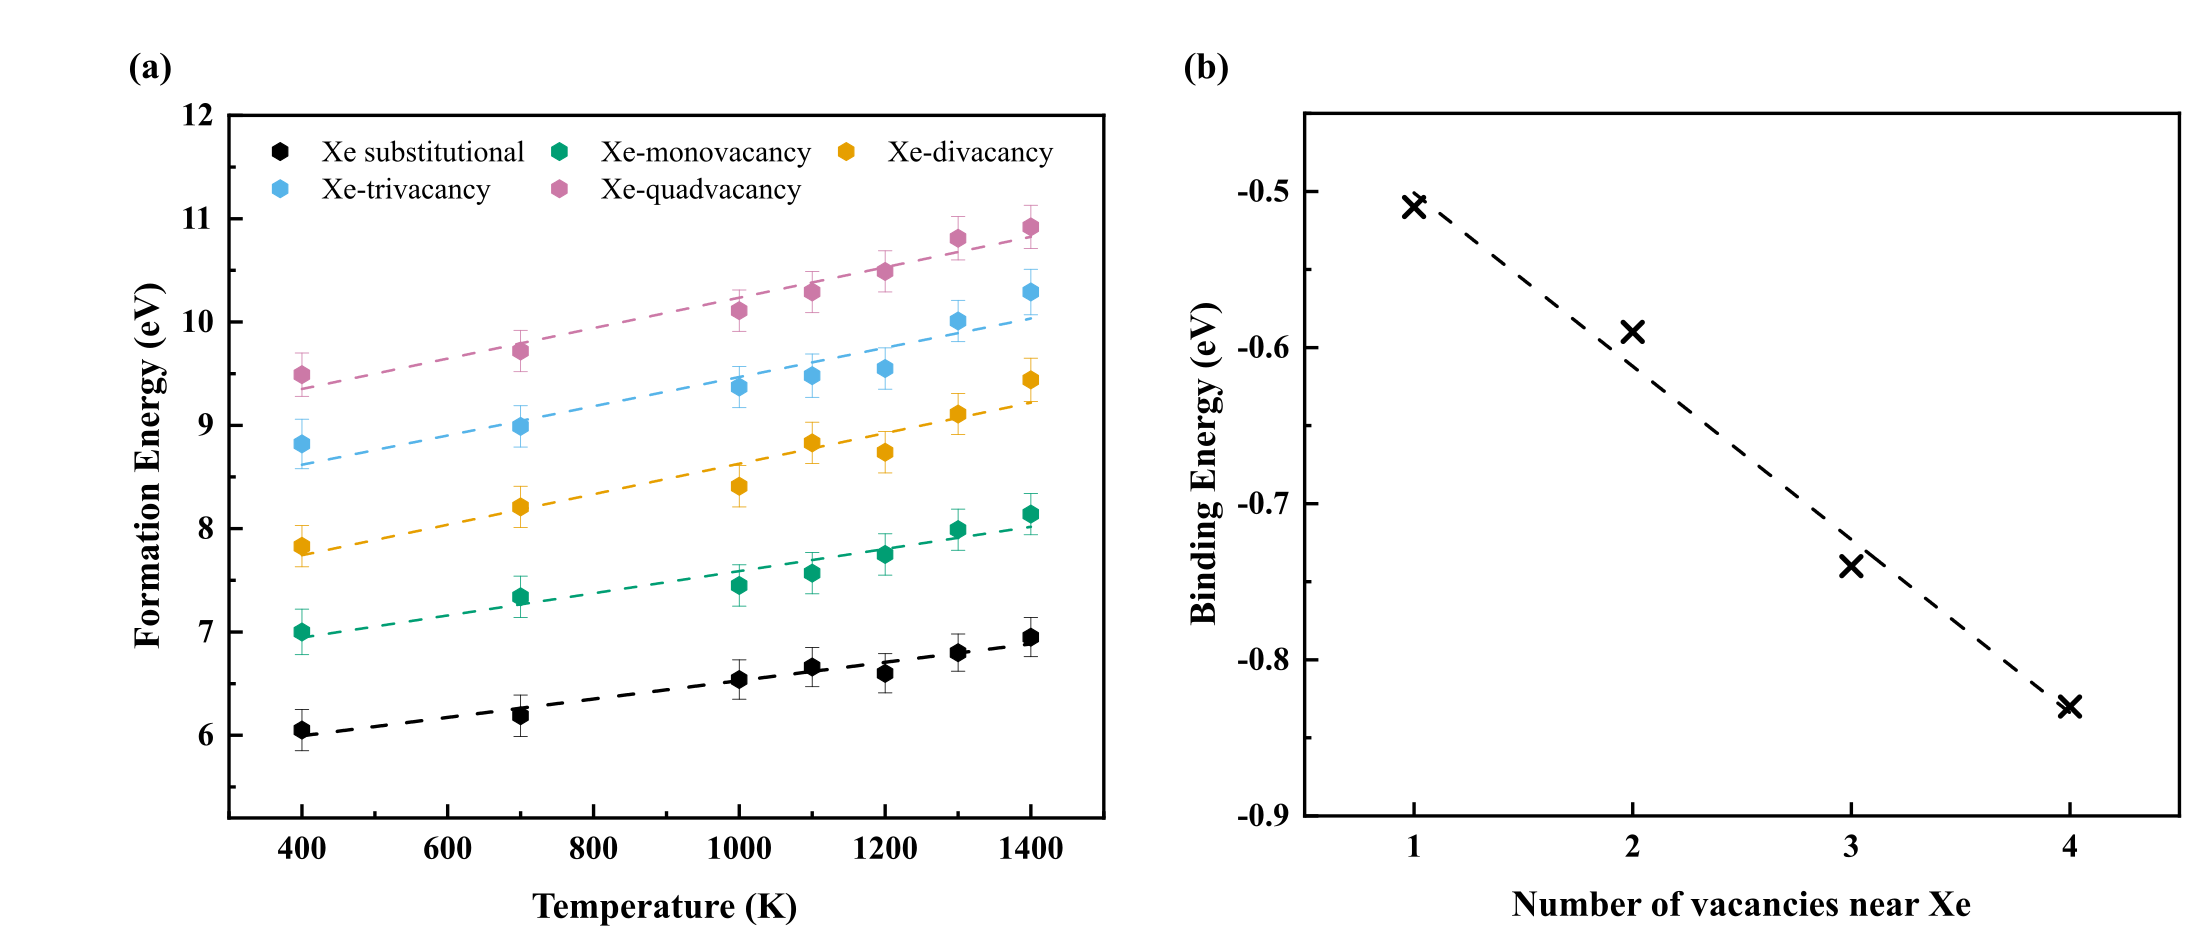
\includegraphics[width=1\textwidth]{Fig7.png}
\caption{(a) Formation energies of Xe-vacancy clusters as a function of temperature. (b) Binding energies of \textit{n}$^{th}$ vacancy in a Xe clusters containing $\it{n}$ vacancy(ies) at 1000 K, where n= 1, 2, 3, and 4 as an example.}
\label{fig:FEBE77}
\end{figure}

Given the formation energies and binding energies of all Xe-vacancy clusters of interest, the absorption and emission coefficients in Eqns. \ref{eq:beta} and \ref{eq:alpha} can be determined and the rate-theory formulation outlined in Eqns. \ref{eqn:Xe_rate1}-\ref{eqn:Xe_rate7} can be implemented. The steady-state concentrations of defects, including vacancies, interstitials, Xe substitutionals, and Xe-vacancy clusters, are calculated as a function of inverse temperature at three fission rate densities in Fig. \ref{fig:Xecon}. The temperature interval was 50 K in the range above 700 K, and the interval was decreased to 25 K below 700 K to show the smooth transition in the defect concentrations. The concentration of the Xe clusters including vacancies up to only four (quadvacancy) are represented for the sake of simplicity in Fig. \ref{fig:Xecon}. Complete data of the defect concentrations with respect to inverse temperature at three different fission rate densities is included in the Appendix. 

The steady-state concentrations of Xe-vacancy clusters were dependent on the temperature, exhibiting three distinct regimes. In the low-temperature regime, the smallest Xe-vacancy cluster (the Xe-monovacancy cluster) had the highest concentration, followed by the Xe-divacancy cluster, the Xe-trivacancy cluster, and the Xe-quadvacancy cluster. This corresponds to temperatures less or equal to 300 K at 5$\times$10$^{18}$ fiss/m$^{3}$/s, 325 K at 5$\times$10$^{20}$ fiss/m$^{3}$/s, and 400 K at 5$\times$10$^{22}$ fiss/m$^{3}$/s. In the low-temperature regime, there are a sufficient number of vacancies present to allow for clustering due to the low recombination rate constant (Fig. \ref{fig:recomb}(b)). However, a small Xe-vacancy cluster is not able to absorb a large number of vacancies and grow into a bigger vacancy cluster since the diffusion of vacancies is extremely slow. In the intermediate temperature range, there are still a sufficient number of vacancies present, and the diffusion of vacancies is sufficiently high to allow for absorption of vacancies by an existing Xe-vacancy cluster, resulting in the highest concentration of the biggest Xe-vacancy cluster. This intermediate regime corresponds to the temperatures between 325 K and 500 K at 5$\times$10$^{18}$ fiss/m$^{3}$/s, 400 K and 575 K at 5$\times$10$^{20}$ fiss/m$^{3}$/s, and 450 K and 625 K at 5$\times$10$^{22}$ fiss/m$^{3}$/s. In the high-temperature regime, the concentration of all of the existing Xe-vacancy clusters started to decrease as the temperature increased. The population of vacancies was dramatically reduced at high temperatures due to the high recombination rate constant and the high diffusivity leading to Frenkel pair annihilation. Thus, there are not enough residual vacancies to interact with the Xe species. As the temperature increased, the concentration of larger Xe-vacancy clusters decreased more rapidly than the concentration of smaller Xe-vacancy clusters. As a result, the concentration of the biggest Xe-vacancy cluster had the lowest concentration, while the concentration of the smallest Xe-vacancy cluster, Xe-monovacancy cluster, had the highest concentration. The high temperature regime corresponds to temperatures greater than 575 K at 5$\times$10$^{18}$ fiss/m$^{3}$/s, 625 K at 5$\times$10$^{20}$ fiss/m$^{3}$/s, and 700 K at 5$\times$10$^{22}$ fiss/m$^{3}$/s. Thus, these three temperature regimes are delineated by changes in the mobility of vacancies and the temperature dependence of the recombination rate. It should be emphasized that these trends are applicable for all Xe cluster sizes investigated (up to the Xe-tetradecavacancy cluster), as displayed in Fig. \ref{fig:FEBE} for clarity. \\

\begin{figure}[hbt!]
\centering
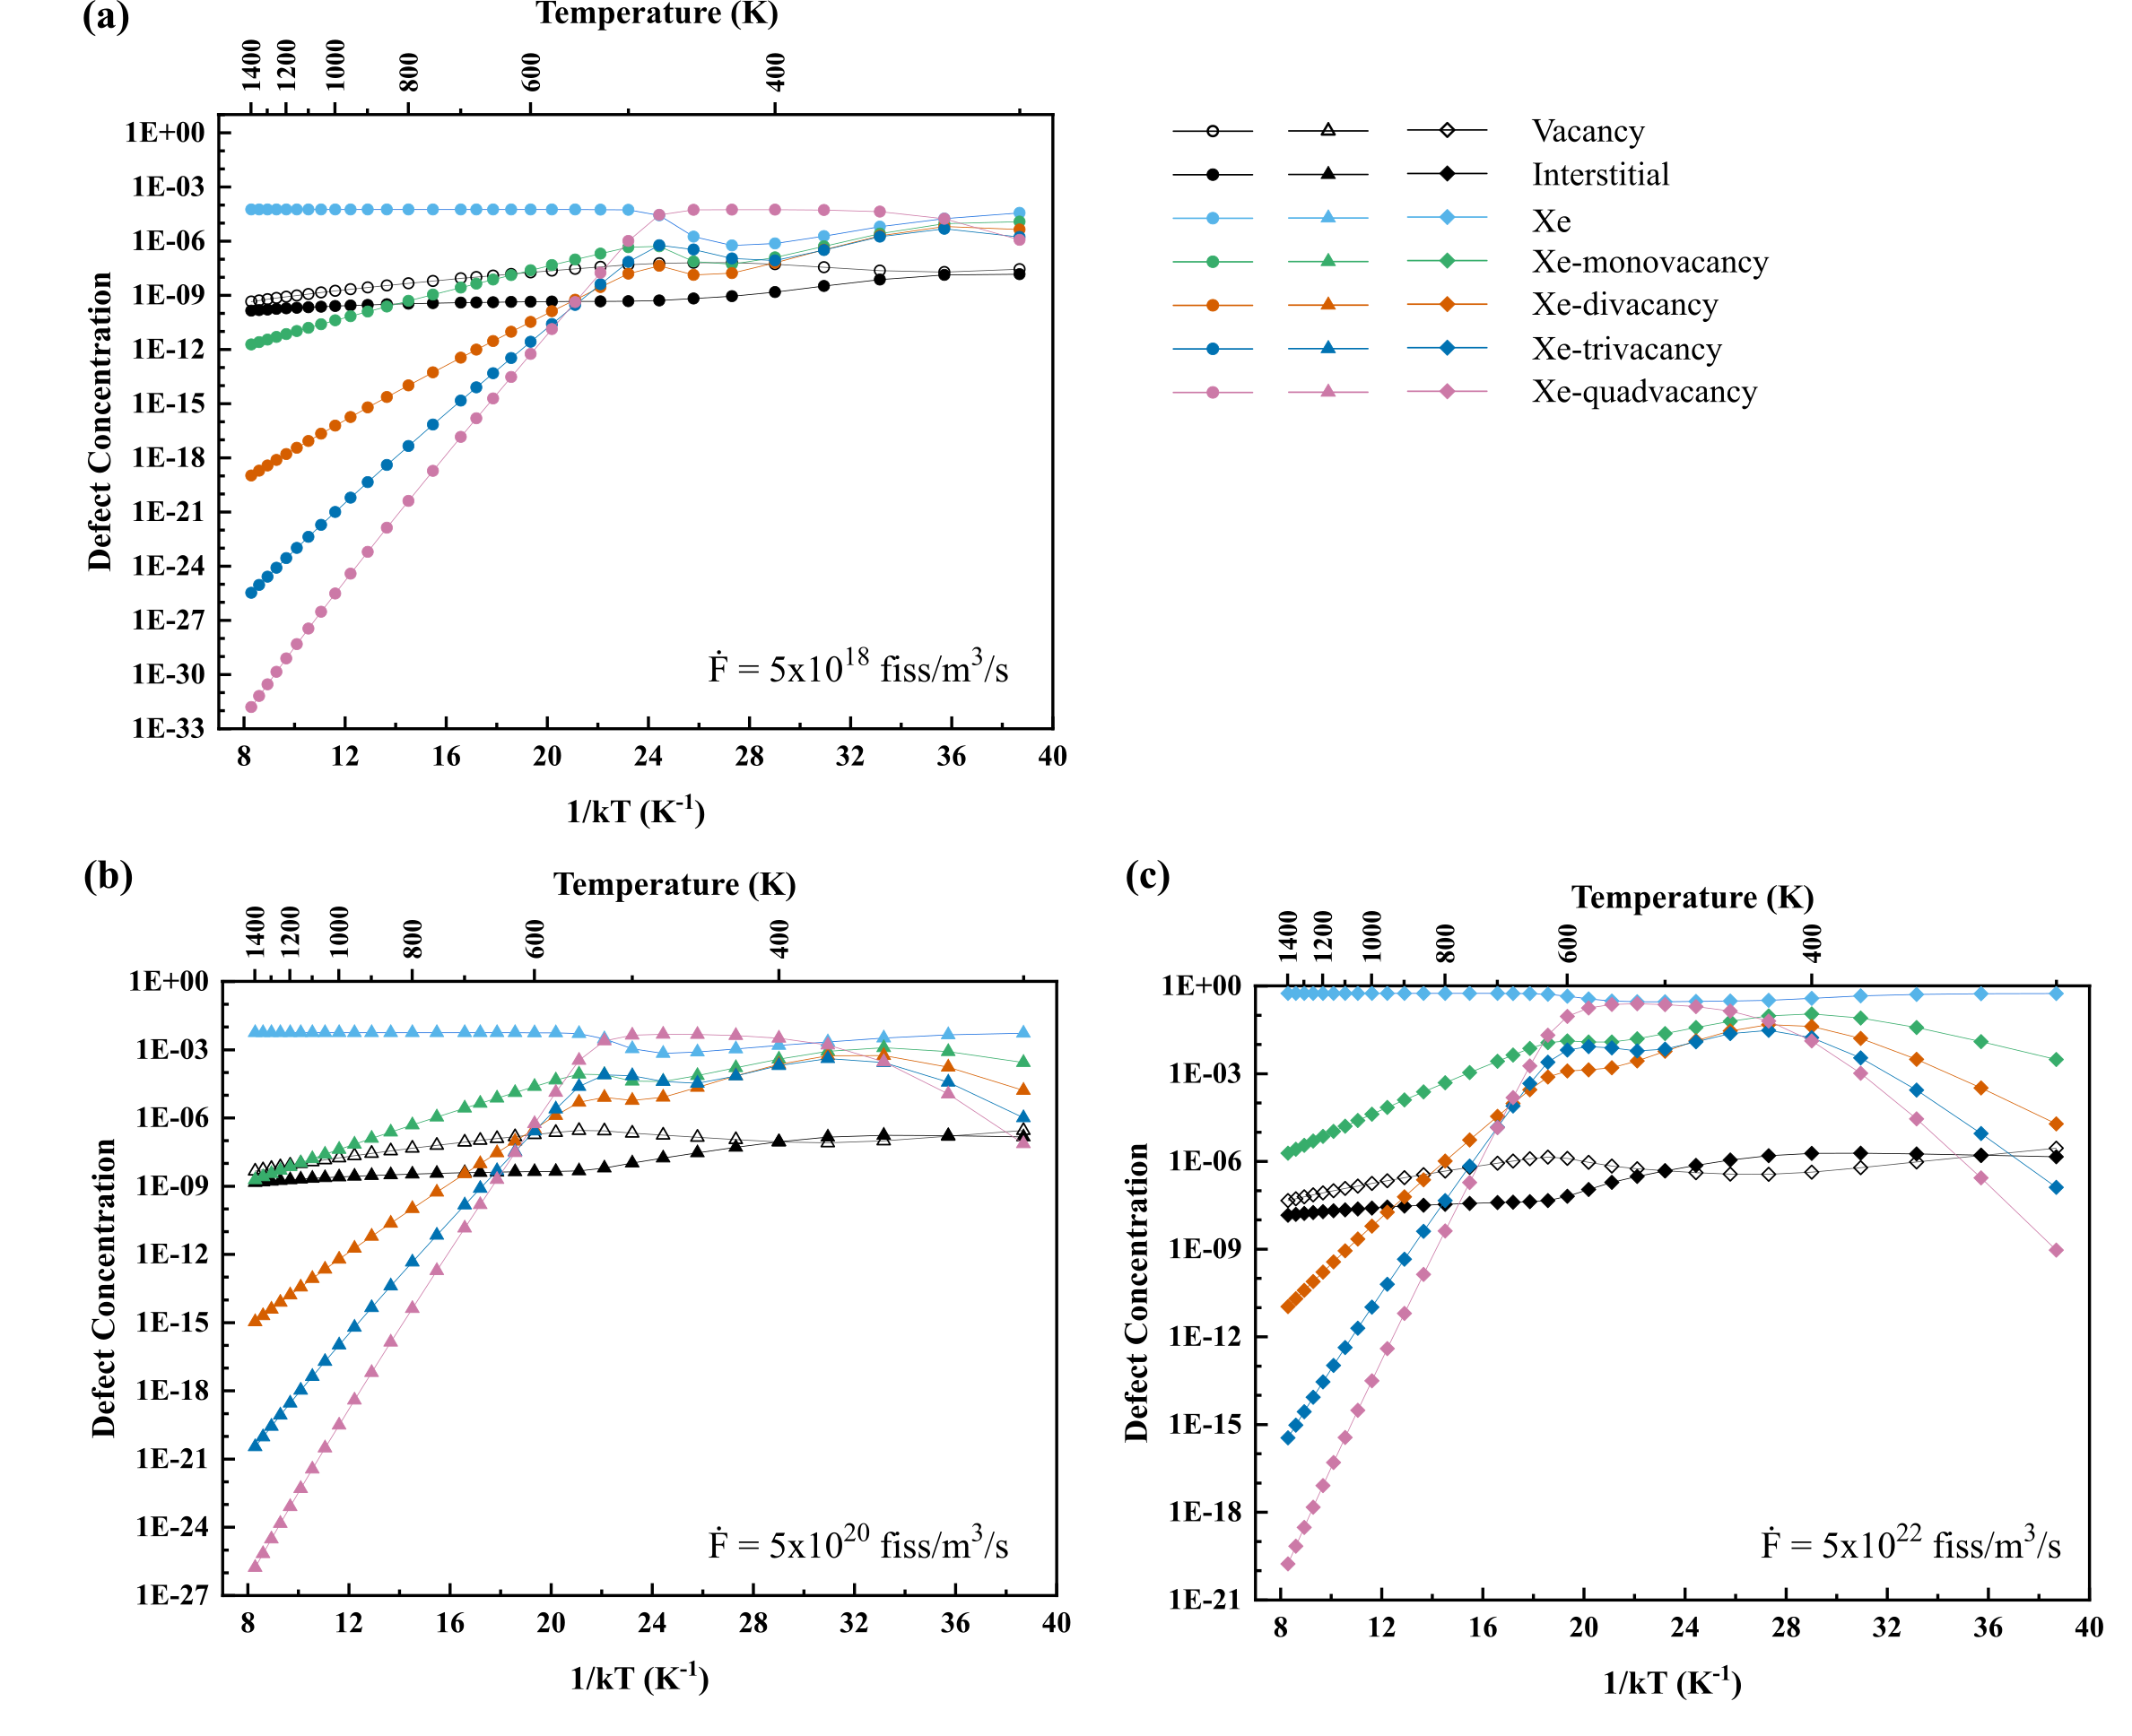
\includegraphics[width=1\textwidth]{Fig8.png}
\caption{Evolution of defect concentrations in $\gamma$U-10Mo as a function of inverse temperature at (a) 5$\times$10$^{18}$ fiss/m$^{3}$/s, (b) 5$\times$10$^{20}$ fiss/m$^{3}$/s, and (c) 5$\times$10$^{22}$ fiss/m$^{3}$/s. Note the differences in the y scales.}
\label{fig:Xecon}
\end{figure}

\FloatBarrier

\indent In order to utilize the Xe-cluster concentrations for Xe radiation-enhanced diffusion calculations in $\gamma$U-10Mo, the individual diffusion coefficients of each cluster must be known, as outlined in Eqn. \ref{eq:surface1}. The diffusion coefficients of Xe in a vacancy cluster with respect to cluster size and temperature as calculated via MD simulations are represented in Fig. \ref{fig:Xediff}(a). The diffusion coefficients of Xe in a vacancy cluster were negligible below 1000 K within the MD timescales. It was expected that the diffusion coefficient of Xe would decrease with increasing vacancy cluster size. However, interestingly, the diffusion coefficients of Xe clusters were effectively independent of the Xe-vacancy cluster size. Due to the insensitivity of the diffusion coefficient on the cluster size, the diffusion coefficient of Xe in a vacancy cluster was obtained by averaging over all cluster sizes at each temperature. The calculated diffusion coefficients were also extrapolated to lower temperatures by fitting to an Arrhenius equation as shown in Fig. \ref{fig:diffcoefficient1}(a) and Table \ref{tab:diff1}. The Xe-vacancy clusters evaluated in this work were not large enough to be immobile. However, since it is known that a large enough Xe-vacancy cluster/bubble is immobile \cite{baker1977migration, kim2022modeling}, the largest cluster described in this work (Xe-tetradecavacancy) was treated as immobile in the radiation-enhanced diffusion calculations to approximate Xe segregation into large bubbles. For example, a 2 nm Xe bubble was found to be immobile in UO$_{2}$ \cite{baker1977migration}. Xe clusters containing more than 14 vacancies were not investigated to identify an immobile Xe-vacancy cluster due to the computational expense associated with conducting MD simulations of complex defects for 500 ns.

\indent The statistical significance of the diffusion was verified in that linear dependencies of the mean-squared displacement as a function of time were achieved for all clusters, and visual inspection via OVITO \cite{stukowski2009visualization} was performed to validate the observed results for the mean-squared displacements. Each individual Xe cluster displayed an Arrhenius relationship, albeit with a different pre-factor and migration energy. It is possible that rapid surface diffusion plays a role in the relative mobility of Xe-clusters with a large ($\it{n}$$>$4) number of vacancies. It should also be noted that only Xe-clusters with a single Xe atom are investigated, and the diffusional behaviors of $m$Xe-$n$vacancy ($\it{m}$$>$1) clusters could be quite different than Xe-vacancy clusters with a single Xe atom. It is presumed that such multi-Xe clusters would diffuse slower than the clusters investigated in this work, and as such the diffusion coefficients within the current study can be considered as an upper bound on the diffusion of possible Xe-vacancy clusters that can form under irradiation. 

\indent The averaged cluster diffusion coefficients from Fig.  \ref{fig:Xediff}(a) and the cluster concentrations from Fig. \ref{fig:Xecon} can now be used to calculate the radiation-enhanced diffusion coefficients of Xe in $\gamma$U-10Mo. These radiation-enhanced diffusivities are represented with respect to inverse temperature at three fission rate densities in Fig. \ref{fig:Xediff}(b). The radiation-enhanced diffusion of Xe is observed to be nearly athermal at high temperatures. Specifically, the athermal regime exists at temperatures greater than or equal to 600 K at 5$\times$10$^{18}$ fiss/m$^{3}$/s, 700 K at 5$\times$10$^{20}$ fiss/m$^{3}$/s, and 800 K at 5$\times$10$^{22}$ fiss/m$^{3}$/s. This is attributed to the decreasing concentration of the smallest Xe-vacancy clusters (Xe-monovacancy), which dominated in this regime, while the diffusion coefficient of Xe in a vacancy cluster increased as the temperature increased. These offsetting contributions resulted in a near-constant radiation-enhanced diffusion of Xe. In the intermediate temperature regime, the radiation-enhanced diffusion of Xe increased with increasing temperature. This was due to the increase of the diffusion coefficient of Xe in a vacancy cluster, while the concentration of the biggest Xe-vacancy clusters (Xe-quadvacancy), which dominated in this regime, remained nearly constant. This tendency  occurred within the temperature range between 350 K and 600 K at 5$\times$10$^{18}$ fiss/m$^{3}$/s, 375 K and 700 K at 5$\times$10$^{20}$ fiss/m$^{3}$/s, and 400 K and 800 K at 5$\times$10$^{22}$ fiss/m$^{3}$/s. In the low-temperature regime, when compared to the intermediate temperature regime, the radiation-enhanced diffusion of Xe increased more rapidly with increasing temperature since both the diffusion coefficient of Xe and the concentration of the smallest Xe-vacancy clusters (Xe-monovacancy), which dominated in this regime, increased. This behavior applied to temperatures less than or equal to 350 K at 5$\times$10$^{18}$ fiss/m$^{3}$/s, 375 K at 5$\times$10$^{20}$ fiss/m$^{3}$/s, and 400 K at 5$\times$10$^{22}$ fiss/m$^{3}$/s.\\

\begin{figure}[hbt!]
\centering
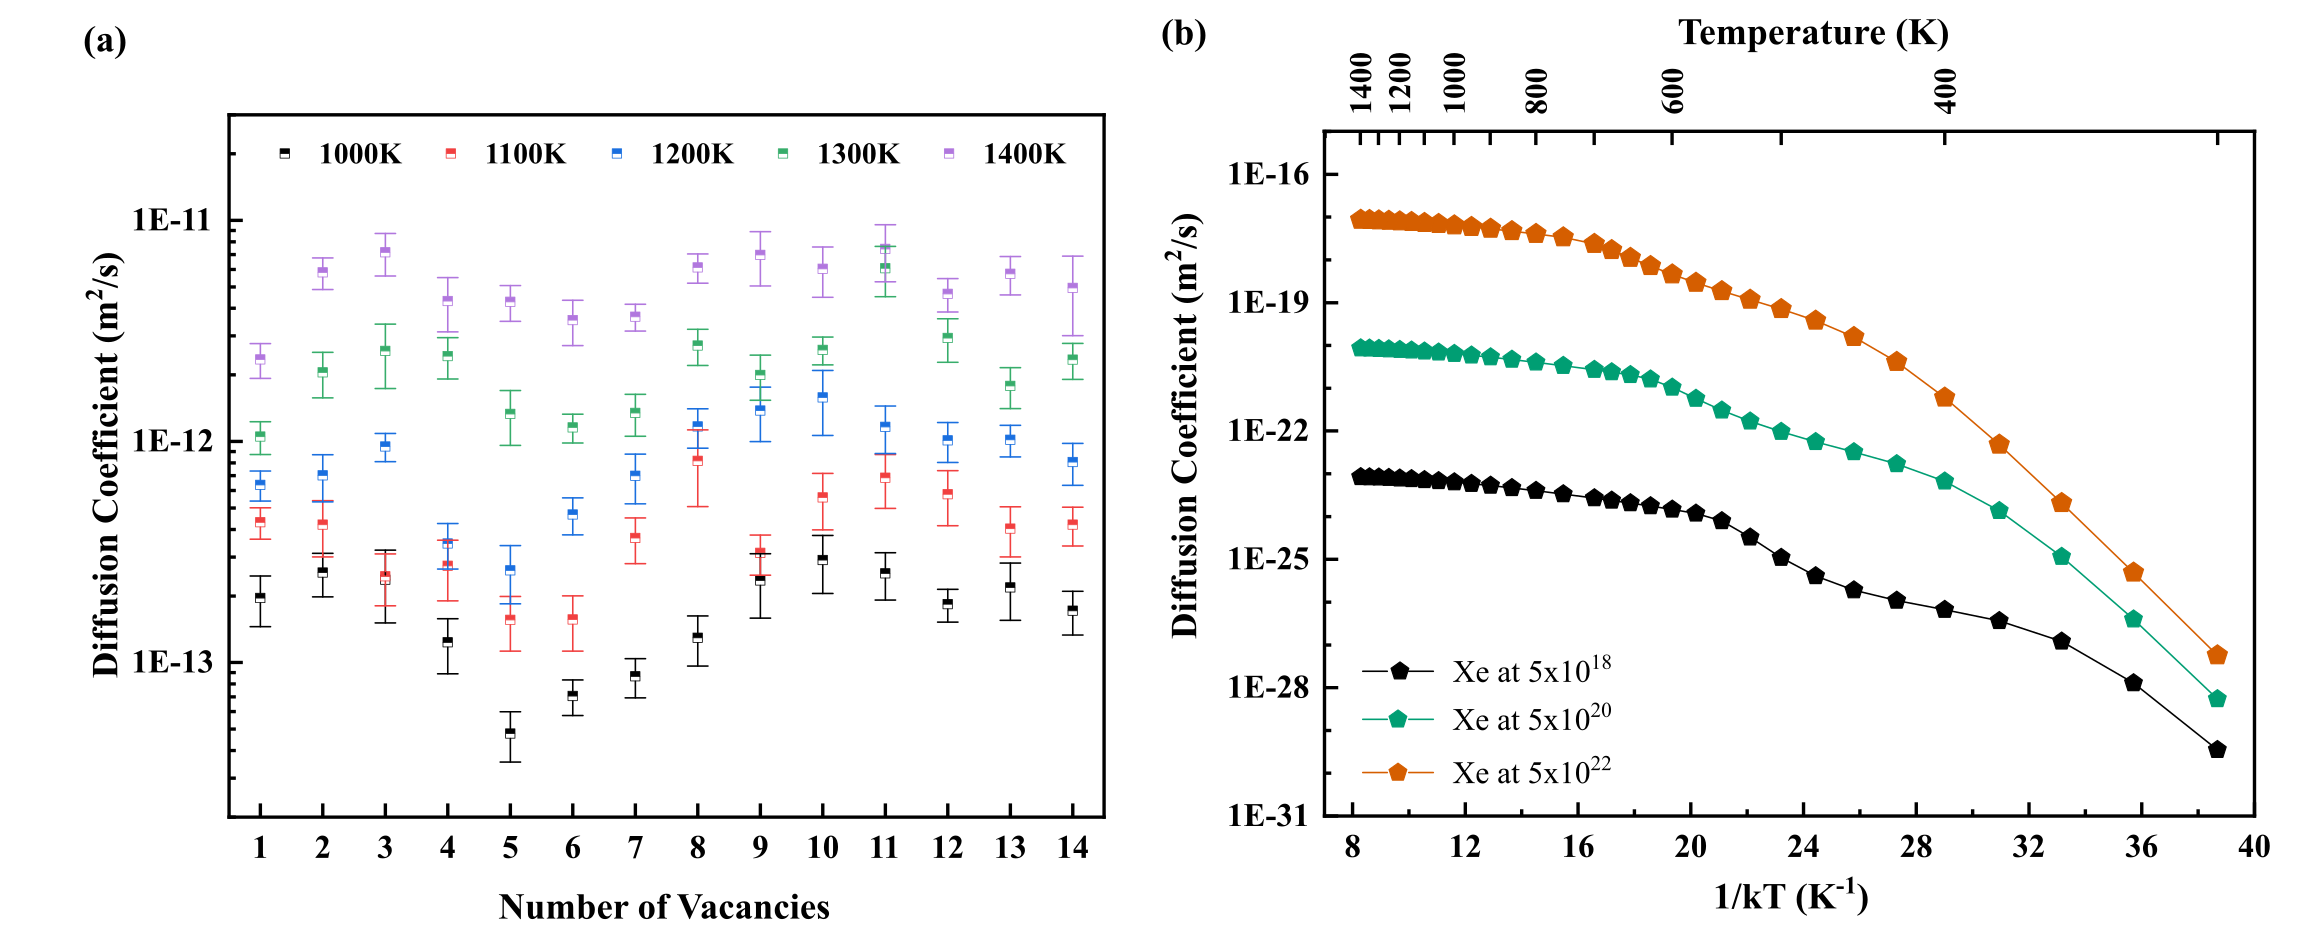
\includegraphics[width=1\textwidth]{Fig9.png}
\caption{(a) Diffusion coefficient of a Xe-vacancy cluster with respect to size. (b) Radiation-enhanced diffusion of Xe in $\gamma$U-10Mo as a function of fission rate density (units are fiss/m$^{3}$/s). }
\label{fig:Xediff}
\end{figure}

\FloatBarrier


\indent The radiation-enhanced diffusion of Xe is plotted along with the intrinsic thermal diffusion and radiation-driven diffusion of Xe in Fig. \ref{fig:Xered} (a)-(c), and the total diffusion coefficient of Xe under irradiation is represented in Fig. \ref{fig:Xered}(d), all as a function of inverse temperature at three fission rate densities. It should be noted that the intrinsic Xe diffusion coefficients, both the previously assumed \cite{hu2016microstructural, Beeler2018microstructural} and calculated in this work, are represented in Fig. \ref{fig:Xered}. The influence of the radiation-enhanced diffusion of Xe on the total diffusion was dependent on the fission rate density and the intrinsic thermal diffusion of Xe. The intrinsic thermal diffusion of Xe, calculated in this work, had a higher activation energy and was two to ten orders of magnitude slower than the previously assumed intrinsic thermal diffusion of Xe depending on the temperature (Fig. \ref{fig:Xered}) \cite{hu2016microstructural, Beeler2018microstructural}. The results of the Arrhenius fits of the intrinsic thermal diffusion of Xe are compared in Table \ref{tab:diff3}. 

Utilizing the intrinsic thermal diffusion of Xe calculated in this work, the radiation-enhanced diffusion of Xe at 5$\times$10$^{18}$ fiss/m$^{3}$/s (Fig. \ref{fig:Xered}(a)) did not significantly contribute to the total diffusion of Xe at the investigated temperatures. For instance, the radiation-enhanced diffusion of Xe was approximately 30-100 times slower than the radiation-driven diffusion of Xe above 700 K.  The intrinsic thermal diffusion of Xe began to dominate the diffusion processes above 950 K, whereas the radiation-driven diffusion of Xe began to dominate below 950 K. For the fission rate density of 5$\times$10$^{20}$ fiss/m$^{3}$/s (Fig. \ref{fig:Xered}(b)), the intrinsic thermal diffusion of Xe dominated above 1150 K and the radiation-driven diffusion of Xe dominated below 1150 K. However, the contribution of the radiation-enhanced diffusion of Xe to the total diffusion increased as the fission rate density increased to 5$\times$10$^{20}$ fiss/m$^{3}$/s (Fig. \ref{fig:Xered}(b)). Specifically, the radiation-enhanced diffusion of Xe was slower than the radiation-driven diffusion of Xe by only a factor of 3-10 above 700 K. As the fission rate density increased further to 5$\times$10$^{22}$ fiss/m$^{3}$/s (Fig. \ref{fig:Xered}(c)), the radiation-enhanced diffusion of Xe exceeded both the intrinsic thermal diffusion and the radiation-driven diffusion of Xe at temperatures above 700 K. \\
\indent The radiation-enhanced diffusion and the radiation-driven diffusion of Xe were also compared to the previously utilized intrinsic thermal diffusion of Xe \cite{hu2016microstructural, Beeler2018microstructural}. Since this estimate for intrinsic diffusion is significantly faster than the values calculated in this work, the temperature range where intrinsic diffusion becomes dominant occurs at a consistently lower temperature for all fission rate densities. Radiation-enhanced diffusion was not a dominant mode of diffusion for any temperatures for the fission rates of 5$\times$10$^{18}$ and 5$\times$10$^{20}$ fiss/m$^{3}$/s. As the fission rate density increased further to 5$\times$10$^{22}$ fiss/m$^{3}$/s (Fig. \ref{fig:Xered}(c)), the radiation-enhanced diffusion of Xe exceeded the intrinsic thermal diffusion and the radiation-driven diffusion of Xe in the temperature range between 700 K to 1100 K. Thus, the previously utilized Xe diffusion assumptions underestimate the potential importance of radiation-enhanced diffusion. 

\indent The differences in the radiation-affected diffusion of U and Mo as compared to Xe are quite stark, especially when considering the respective trends as a function of the fission rate. As mentioned previously, in both U and Mo, a square-root and linear relationship were observed in the radiation-enhanced diffusion and radiation-driven diffusion with respect to fission rate density, respectively. However, in the case of Xe, it becomes more complicated due to the interaction of vacancies with Xe and Xe-vacancy clusters, which created non-uniform variability as a function of fission rate density and temperature. 
\\

\begin{figure}[hbt!]
\centering
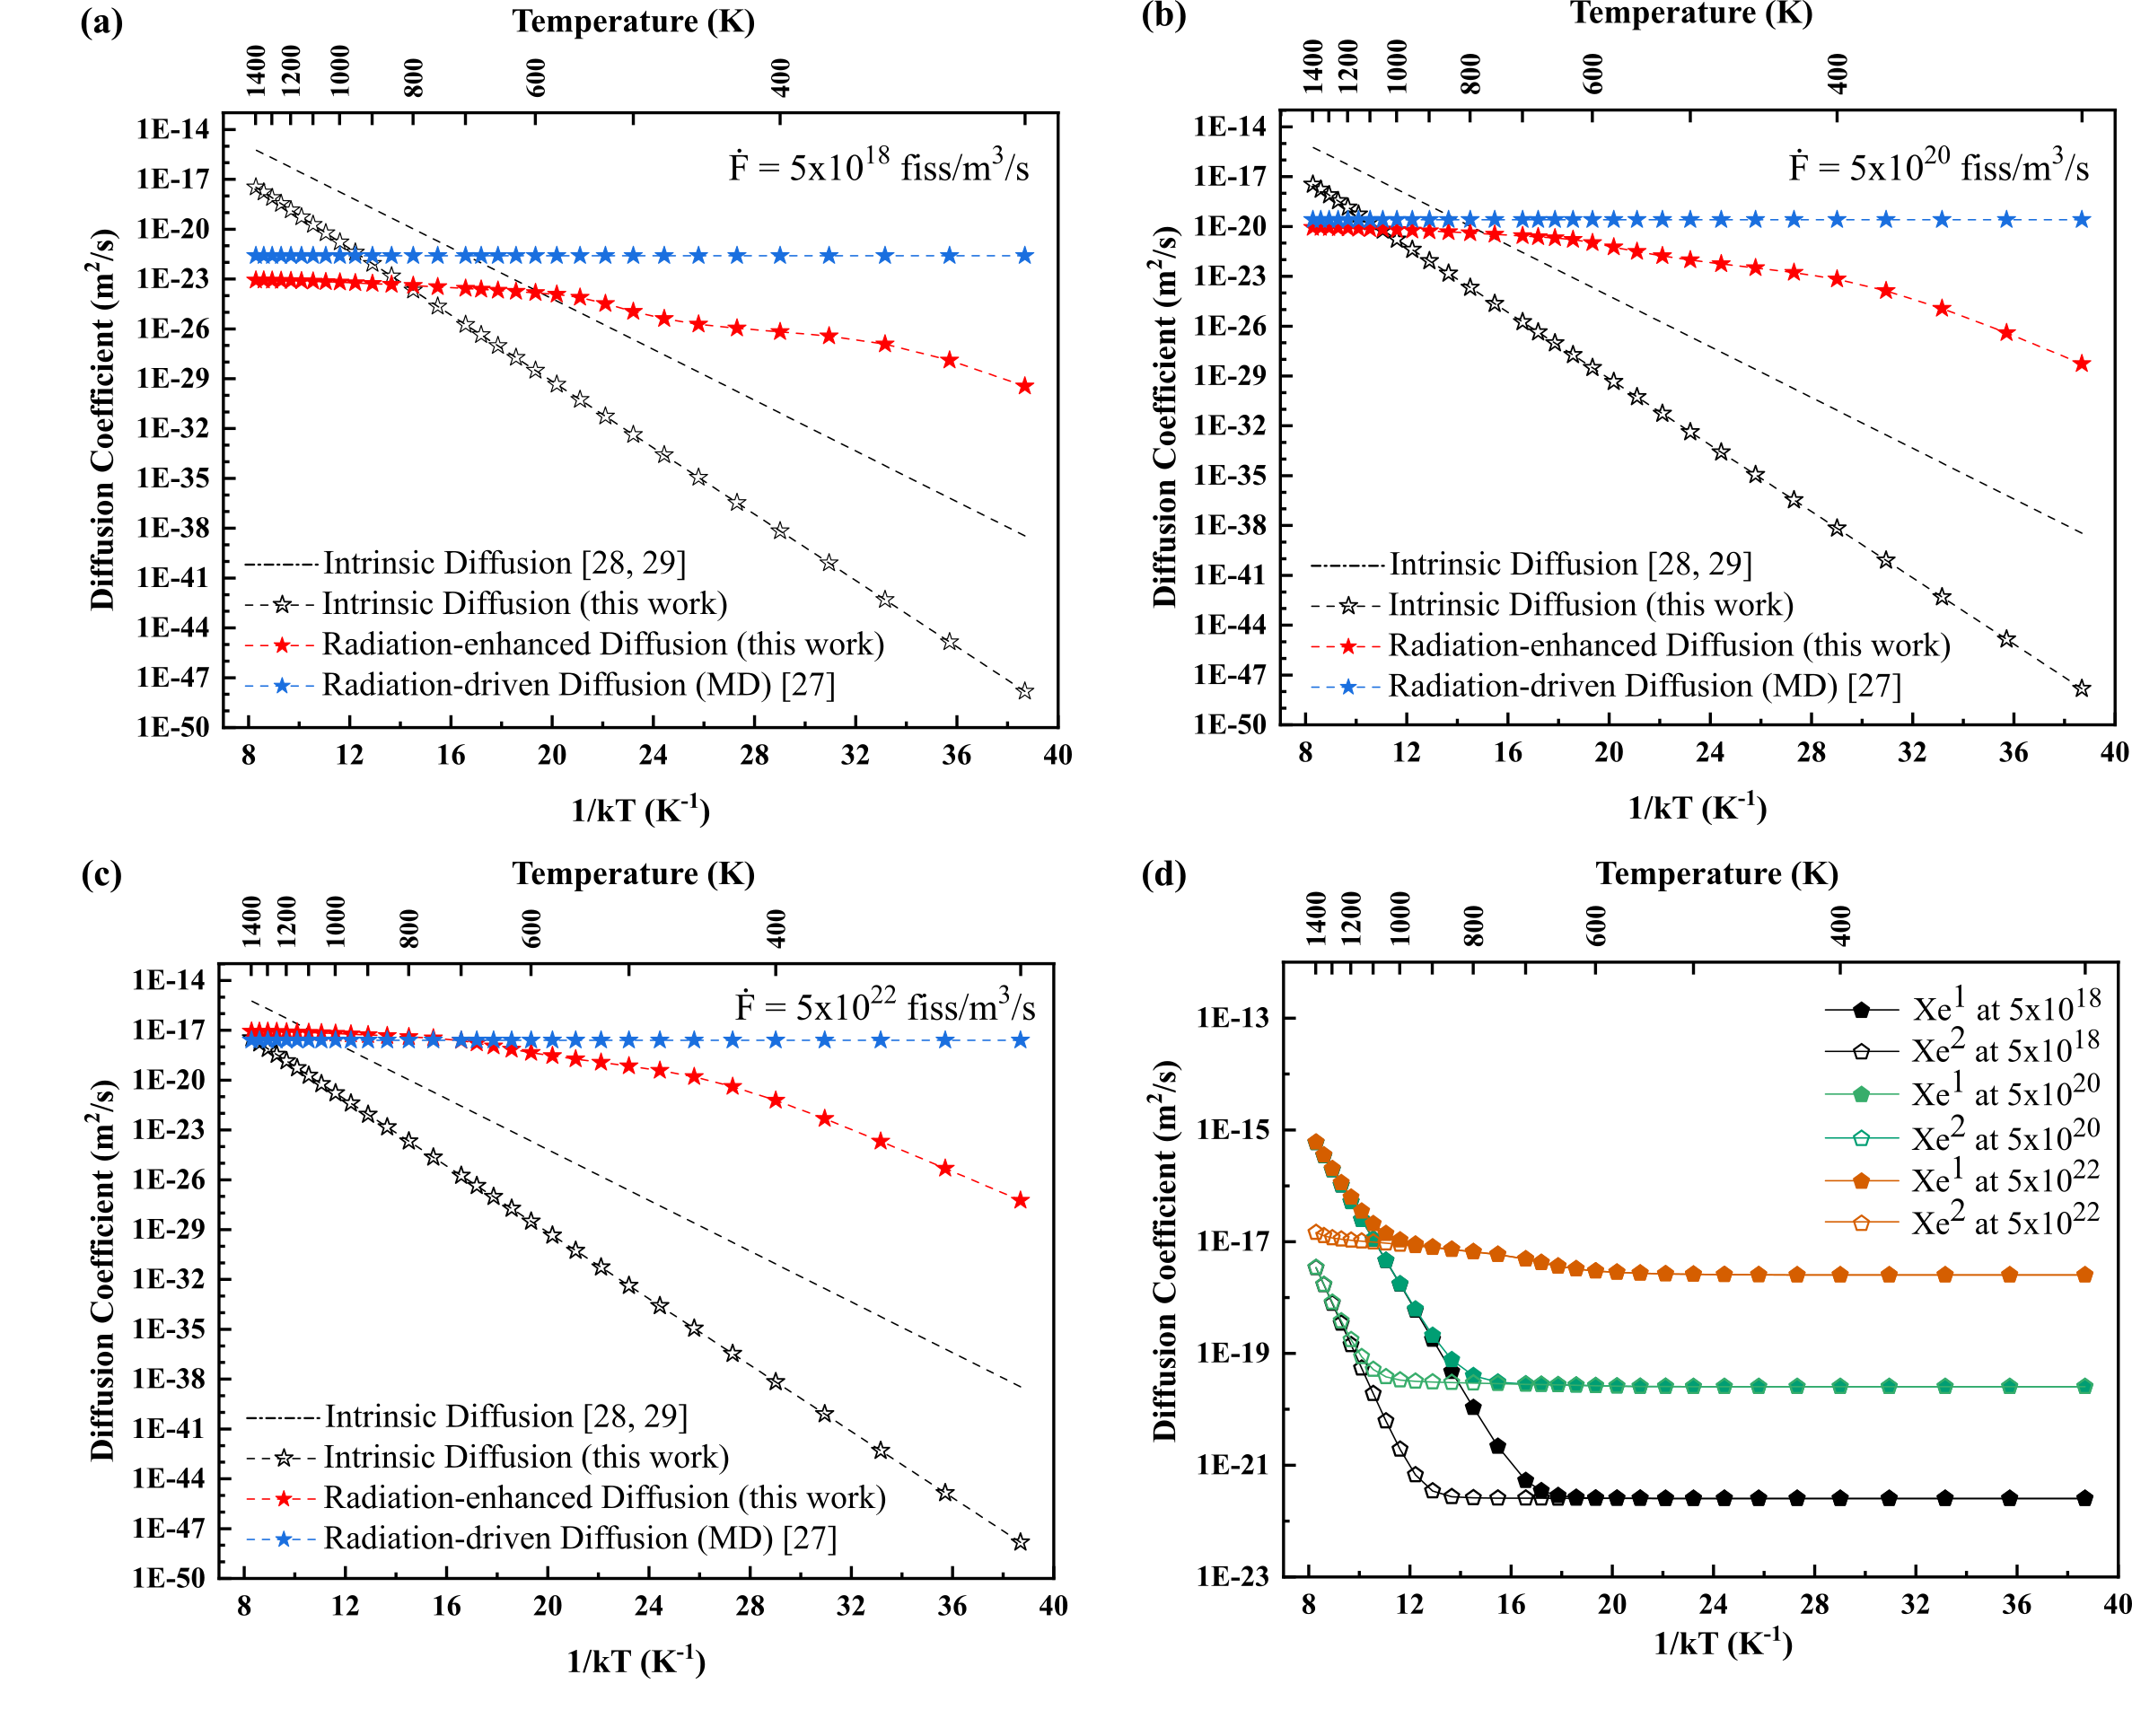
\includegraphics[width=1\textwidth]{Fig10.png}
\caption{Intrinsic diffusion, radiation-driven diffusion, and radiation-enhanced diffusion of Xe in $\gamma$U-10Mo at (a) 5$\times$10$^{18}$ fiss/m$^{3}$/s, (b) 5$\times$10$^{20}$ fiss/m$^{3}$/s, and (c) 5$\times$10$^{22}$ fiss/m$^{3}$/s. (d) Total diffusion of Xe as a function of fission rate density (fiss/m$^{3}$/s). Note the differences in the y scales. Xe$^{1}$ is calculated from the previous assumption, and Xe$^{2}$ is calculated in this work \cite{hu2016microstructural, Beeler2018microstructural}.}
\label{fig:Xered}
\end{figure}


\begin{table}[hbt!]
\captionsetup{font=normalsize} 
\caption{Arrhenius fit of intrinsic thermal diffusion of Xe in $\gamma$U-10Mo.}
\renewcommand{\arraystretch}{1.25}
\begin{center}
\begin{tabular}{cccc}
\hline
 & Activation energy (eV) & Pre-exponential factor (m$^{2}$/$\mathrm{s}$)  \\ 
\hline
Previous assumption \cite{hu2016microstructural, Beeler2018microstructural} & 1.76 & 1.28$\times$10$^{-9}$ \\  
This work & 2.30 & 6.53$\times$10$^{-10}$ \\
\hline
\end{tabular}
\end{center}
\label{tab:diff3} 
\end{table} 

\FloatBarrier

\section{Discussion}
\label{sec:Discussion}
\indent Radiation-enhanced diffusion of Xe behaved differently as compared to radiation-enhanced diffusion of U and Mo with respect to temperature and fission rate density in $\gamma$U-10Mo. The intrinsic thermal diffusion, radiation-enhanced diffusion, and radiation-driven diffusion of U and Mo dominated in the high, intermediate, and low-temperature regimes, respectively, depending on the fission rate density as described in Section \ref{sec:RED_UMo}. Given that the reactor operating temperature is below approximately 150$^{\circ}$C and the fission rate density is on the order of 10$^{20}$ fiss/m$^{3}$/s in research reactors, both radiation-enhanced diffusion and radiation-driven diffusion of U and Mo contribute to species mobility under irradiation at all relevant research reactor temperatures and fission rate densities \cite{meyer2014irradiation, marshall2016new}. On the other hand, the radiation-enhanced diffusion of Xe did not significantly impact the diffusion under irradiation at relevant temperatures and fission rate densities in research reactors. Alternately, radiation-driven diffusion of Xe dominated the diffusion process of Xe for relevant operating conditions in research reactors. For the establishment of future models, the intrinsic thermal diffusion of each element can likely be neglected in research reactors due to the specific operating parameters (temperature and fission rate density) which dictate the prevalence of irradiation-assisted diffusion.

\indent Radiation-enhanced diffusion was previously investigated in other fuel materials such as UO$_{2}$ \cite{cooper2021irradiation, andersson2014atomistic} and U$_{3}$Si$_{2}$ \cite{matthews2020cluster}. In UO$_{2}$, it was observed that radiation-enhanced diffusion of Xe dominated over the intrinsic thermal diffusion of Xe below 1561 K at the fission rate density of 10$^{19}$ fiss/m$^{3}$/s from experiments \cite{turnbull1982diffusion}, which is inconsistent with the Xe observations in this work. Anderson et al. \cite{andersson2014atomistic} predicted the radiation-enhanced diffusion of Xe via cluster dynamics parametrized by DFT and MD simulations, which agreed well with experimental observations. For example, the radiation-enhanced diffusion of Xe dominated over the intrinsic diffusion of Xe below 1771 K at the identical fission rate density in UO$_{2}$ \cite{turnbull1982diffusion, andersson2014atomistic}. In addition, the radiation-enhanced diffusion of U in UO$_{2}$ dominated between 1250 K and 1800 K at 10$^{19}$ fiss/m$^{3}$/s \cite{matthews2020cluster}. This work established credibility for the prediction of Xe radiation-enhanced diffusion via strictly computational pathways. In the U$_{3}$Si$_{2}$ system, radiation-enhanced diffusion of U and Si did not significantly contribute to the total diffusion at the evaluated fission rate densities from 10$^{17}$ fiss/m$^{3}$/s to 10$^{19}$ fiss/m$^{3}$/s \cite{cooper2021irradiation}, which is in qualitative agreement with the behavior of Xe in this work. The radiation-driven diffusion of U and Si was greater than the radiation-enhanced diffusion of U and Si by 4-5 orders of magnitude \cite{cooper2021irradiation}. Uranium diffusion was faster than Si diffusion, and diffusion occurred primarily via interstitials rather than vacancies in U$_{3}$Si$_{2}$ \cite{cooper2021irradiation, andersson2019density}. The relative similarities of U-10Mo to the U$_{3}$Si$_{2}$ system, specifically both having metallic bonding and interstitial-based self-diffusion, suggest that the irradiation-affected diffusion behaviors would also show some similarities, which is confirmed in this work.

\indent  A comment should be made to contextualize some of the assumptions made, and some of the results observed, in this work. To calculate the radiation-enhanced diffusion of Xe, rate-theory equations (Eqs. 13-19) were constructed to calculate the steady-state concentrations of defects, comprising vacancies, interstitials, Xe, and Xe-vacancy clusters in the fuel under irradiation. However, unlike the concentrations of vacancies and interstitials, the concentrations of Xe-vacancy clusters did not reach a steady-state value since Xe was continuously produced, and only small Xe-vacancy clusters were considered in the rate-theory equations. Experimentally, it is expected that the concentration of Xe will increase with respect to time under irradiation since Xe is continually produced via fission, but fission gas release does not occur in the U-Mo fuel system. Thus, the concentrations at the time of 45 days, which is approximately the time at which U-10Mo fuel undergoes recrystallization in research reactors, are utilized in the determination of radiation enhanced diffusion of Xe \cite{kim2013recrystallization, leenaers2016high, perez2012rertr1,perez2012rertr2, smith2022high}. In addition, the presence of large fission gas bubbles is not explicitly taken into account in the rate-theory equations. Point defects (vacancies and interstitials) and Xe will diffuse into fission gas bubbles, as well as grain boundaries, which are the primary sinks in the fuel, and losses of point defects and Xe will likely decrease the Xe-vacancy cluster concentrations under irradiation. Thus, this work represents an upper bound of the possible radiation-enhanced diffusion of Xe, with a series of assumptions that likely exaggerate the rate at which Xe and Xe-vacancy clusters are able to be transported in U-Mo fuel. This, combined with the limited range of prevalence of radiation-enhanced diffusion for Xe in U-Mo, indicates that it is highly likely that the radiation-driven diffusion of Xe will be the dominant mode of Xe diffusion at temperatures relevant to research reactors.\\

\section{Summary and Conclusions}
In the present work, the radiation-enhanced diffusion coefficients of U, Mo, and Xe in $\gamma$U-10Mo were calculated using rate-theory models and MD simulations with the ternary U-Mo-Xe interatomic potential \cite{smirnova2013ternary} in the temperature range between 300 K and 1400 K and the fission rate density range between 5$\times$10$^{18}$ fiss/m$^{3}$/s and 5$\times$10$^{22}$ fiss/m$^{3}$/s. The calculated radiation-enhanced diffusion coefficient of each element was compared to the intrinsic thermal diffusion and the radiation-driven diffusion, determined previously  \cite{beeler2021radiation, huang2013}. The intrinsic thermal diffusion of Xe was calculated using the concentration of vacancies at equilibrium and the diffusion coefficient of Xe in a monovacancy cluster. The total diffusion of U, Mo, and Xe under irradiation conditions were also determined by summing the radiation-enhanced diffusion, calculated in this work, and the previously determined intrinsic thermal diffusion and radiation-driven diffusion \cite{beeler2021radiation, huang2013}. It was found that both radiation-enhanced diffusion and radiation-driven diffusion of U and Mo dominated at the operating temperatures and typical fission rate densities of research reactors. The influence of the radiation-enhanced diffusion of Xe on the total diffusion of Xe under irradiation increased with increasing fission rate density. However, the radiation-enhanced diffusion of Xe did not significantly contribute to the total diffusion of Xe at a fission rate density of 5$\times$10$^{18}$ fiss/m$^{3}$/s and 5$\times$10$^{20}$ fiss/m$^{3}$/s. The radiation-enhanced diffusion of Xe exceeded the intrinsic diffusion of Xe, calculated in this work, as well as the radiation-driven diffusion of Xe at 5$\times$10$^{22}$ fiss/m$^{3}$/s above 700 K, although, this is likely beyond the fission rate density regime that is obtained within research reactors. The total diffusion coefficients of U, Mo, and Xe in $\gamma$U-10Mo, updated in this work, will be utilized as important parameters in mechanistic fuel models, as well as potentially in other nuclear fuel  mesoscale models, such as kinetic Monte Carlo, phase-field models, cluster dynamics, and finite element analysis, to predict the microstructural evolution under irradiation more accurately. 

\section{CRediT author statement}
\textbf{Gyuchul Park:} Conceptualization, Formal analysis, Software, Investigation, Methodology, Visualization, Writing-original draft. \textbf{Benjamin Beeler:} Conceptualization, Funding acquisition, Methodology,  Project administration, Resources, Supervision, Writing-review and editing. \textbf{Maria A. Okuniewski:} Conceptualization, Funding acquisition, Methodology, Project administration, Resources, Supervision, Writing-review and editing.

\section{Acknowledgements}
This work was supported by the U.S. Department of Energy, Office of Material Management and Minimization, National Nuclear Security Administration, under DOE-NE Idaho Operations Office Contract DE-AC07-05ID14517. This research made use of the High-Performance Computing Center at Idaho National Laboratory, which is supported by the Office of Nuclear Energy of the U.S. Department of Energy and the Nuclear Science User Facilities. 

\clearpage
\appendix
\section{}

\setcounter{figure}{0}

The concentration of vacancies, interstitials, and Xe clusters as a function of inverse temperature at three fission rate densities is shown in Fig. \ref{fig:FEBE}, including data for all Xe-vacancy clusters investigated.

\begin{figure}[hbt!]
\centering
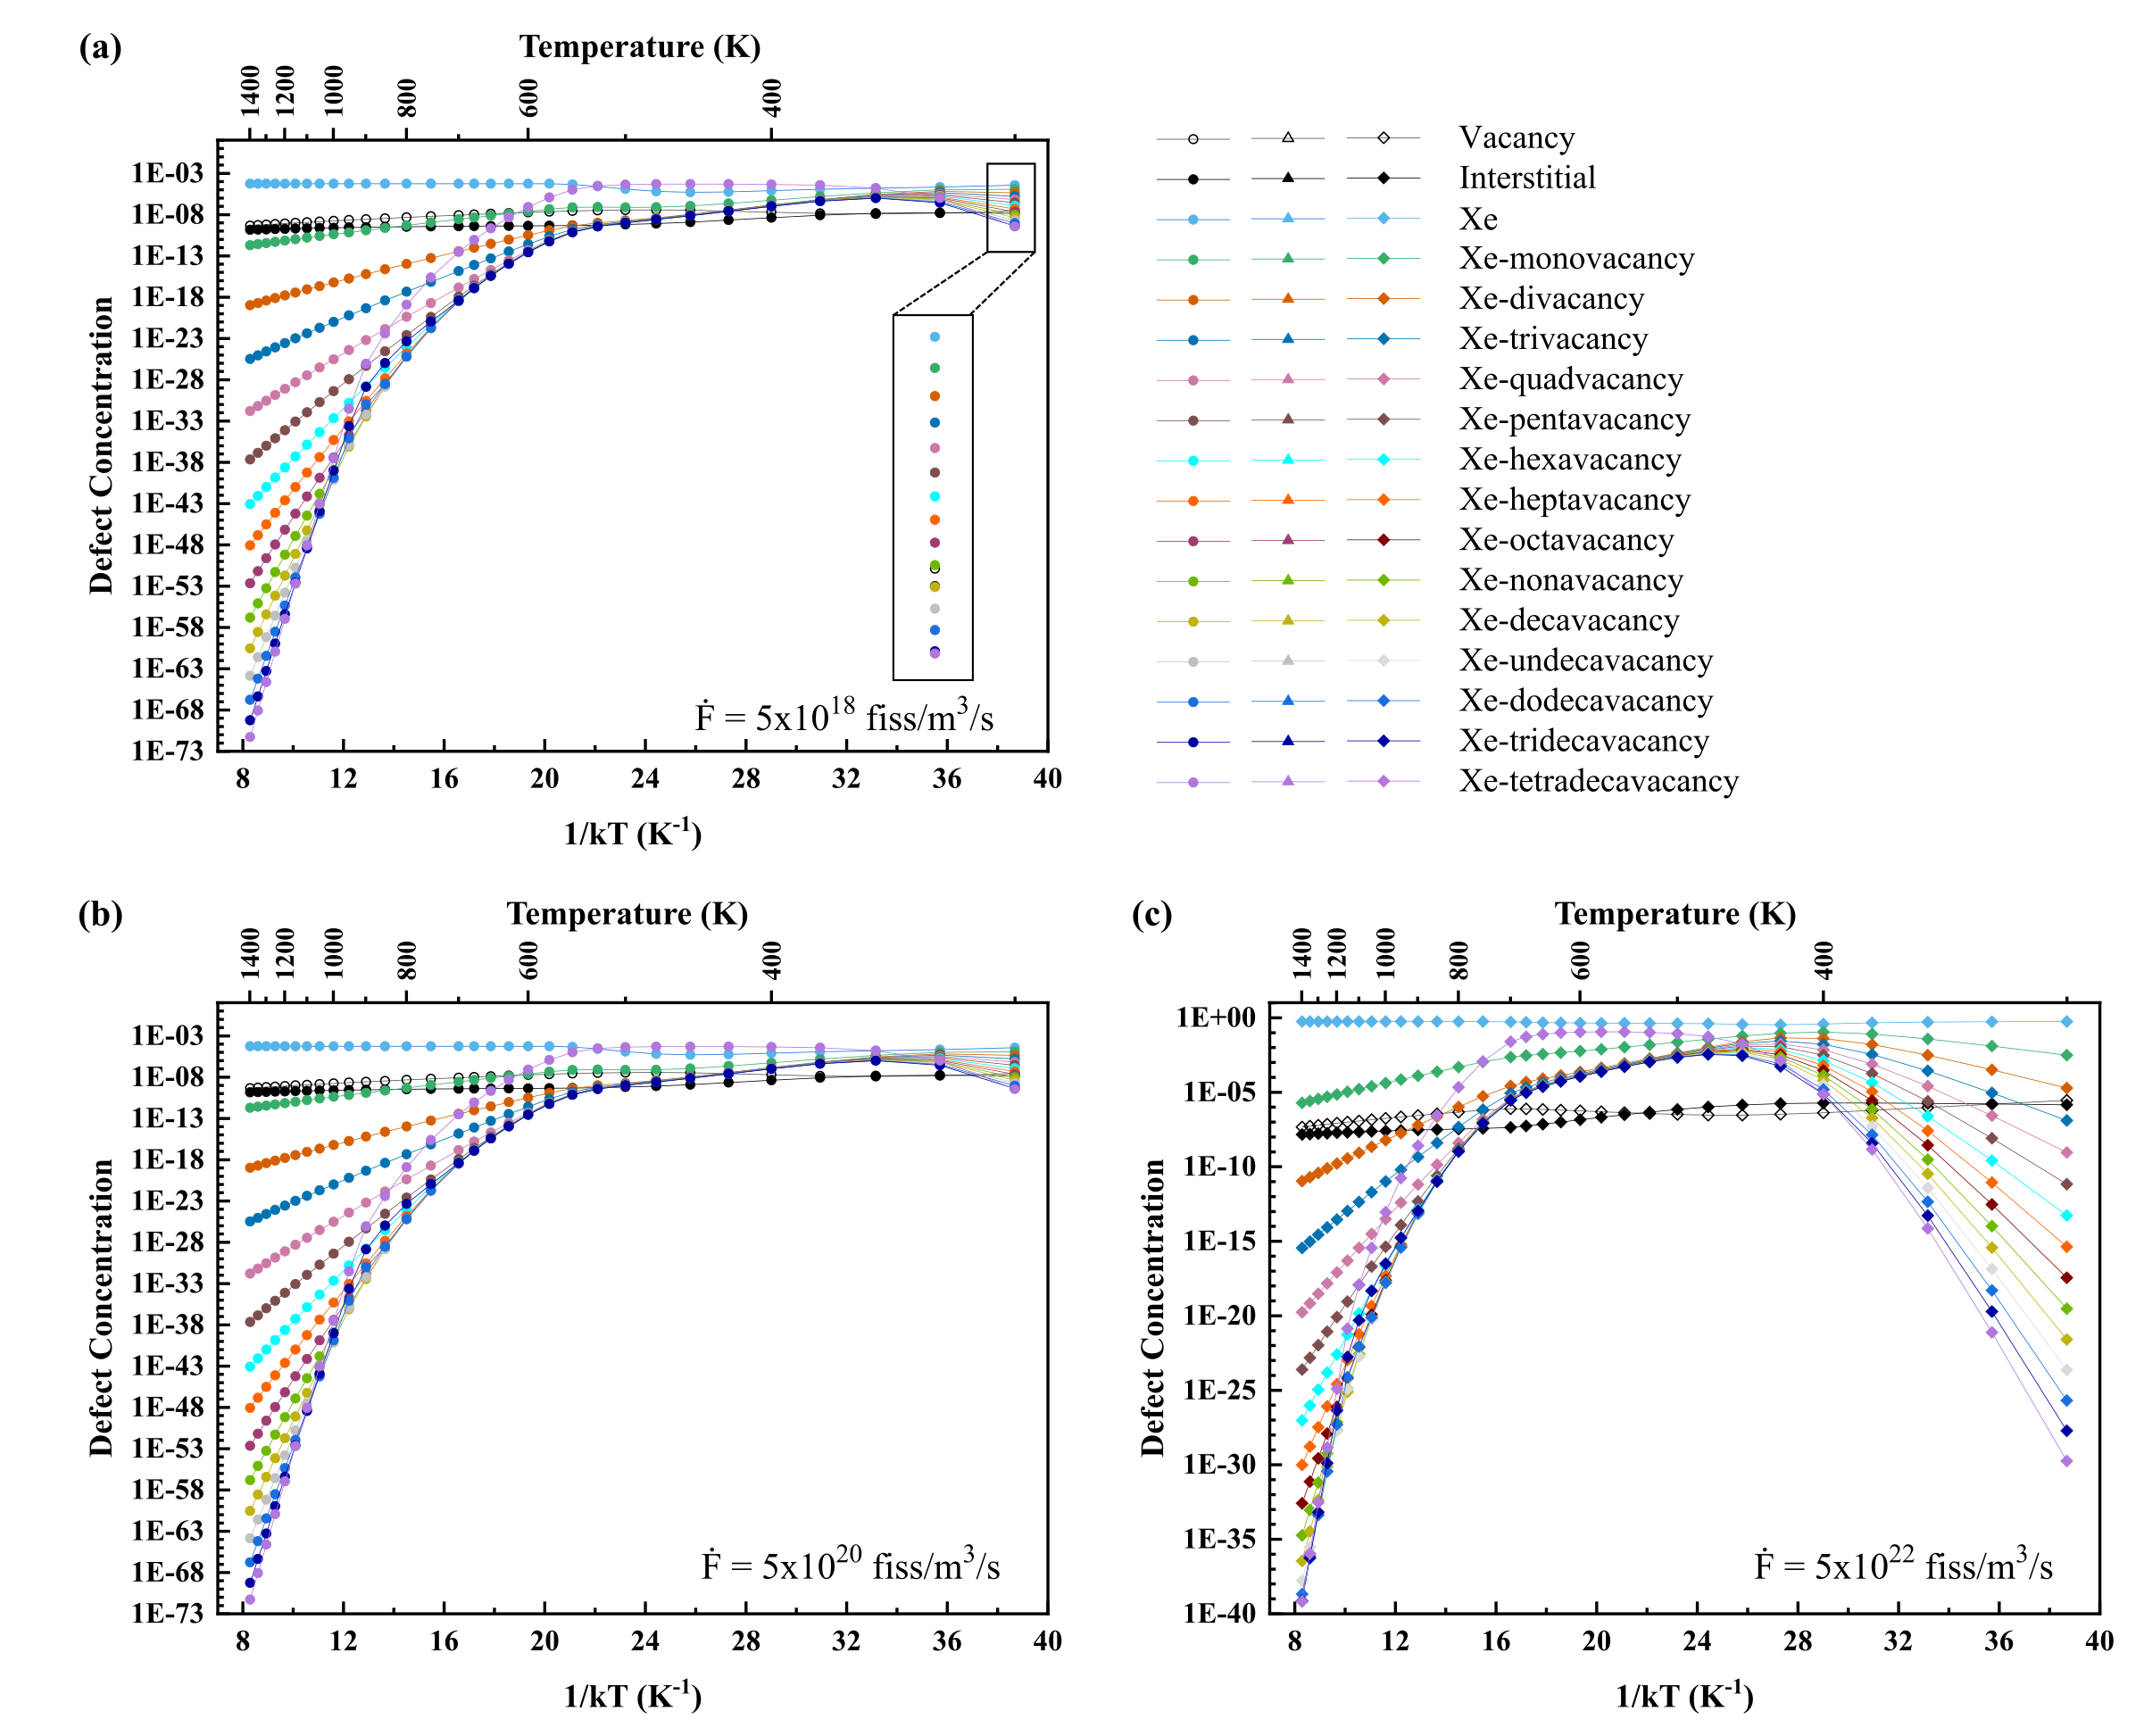
\includegraphics[width=1\textwidth]{A1.png}
\caption{Evolution of concentrations of vacancies, interstitials, Xe, and Xe-vacancy clusters in $\gamma$U-10Mo as a function of inverse temperature at (a) 5$\times$10$^{18}$ fiss/m$^{3}$/s, (b) 5$\times$10$^{20}$ fiss/m$^{3}$/s, and (c) 5$\times$10$^{22}$ fiss/m$^{3}$/s. The Xe-vacancy clusters containing up to 14 vacancies (Xe-tetradecavacancy) are considered.}
\label{fig:FEBE}
\end{figure}
\clearpage
\bibliographystyle{elsarticle-num} 
\bibliography{mybib.bib}
\end{document}
